% Manuscript entry point; content and typography live in the included sources.
% Compile this archived report with make; the conference export lives separately.
\documentclass[11pt,letterpaper]{article}
% Typography and layout for the standalone preprint.
\usepackage[T1]{fontenc}
\usepackage{newtxtext}
\usepackage[varqu,varl,scaled=0.95]{zi4}
\usepackage{amsmath,amssymb,amsthm}
\usepackage{newtxmath}
\usepackage[letterpaper,margin=1in,headsep=18pt]{geometry}
\usepackage{microtype}
\usepackage{booktabs,array}
\usepackage{flafter}
\usepackage{placeins}
\usepackage{xcolor}
\usepackage{graphicx}
\usepackage{tikz}
\usetikzlibrary{arrows.meta,positioning}
\usepackage{pgfplots}
\pgfplotsset{compat=1.18}
\usepackage{listings}
\usepackage{enumitem}
\usepackage{fancyhdr}
\usepackage[font=small,labelfont=bf,labelsep=period,skip=6pt]{caption}
\usepackage[explicit]{titlesec}
\usepackage{url}
\definecolor{ink}{HTML}{214E70}
\definecolor{accent}{HTML}{B85C38}
\definecolor{pale}{HTML}{F3F5F7}
\usepackage[colorlinks=true,linkcolor=ink,citecolor=ink,urlcolor=ink]{hyperref}
\hypersetup{pdftitle={Whole-Pipeline Scheduling for Real-Time Spectral Analysis},pdfauthor={Christian Kauten},pdfsubject={Preprint on whole-pipeline scheduling, exact-hop publication, and execution granularity for real-time spectral analysis},pdfkeywords={FFT, STFT, cooperative scheduling, real-time audio, spectrum analysis, VCV Rack}}

% Section headings: numbered, bold, compact.
\titleformat{\section}{\normalfont\large\bfseries}{\thesection}{0.8em}{#1}
\titleformat{\subsection}{\normalfont\normalsize\bfseries}{\thesubsection}{0.8em}{#1}
\titleformat{name=\section,numberless}{\normalfont\large\bfseries}{}{0pt}{#1}
\titleformat{name=\subsection,numberless}{\normalfont\normalsize\bfseries}{}{0pt}{#1}
\titlespacing*{\section}{0pt}{2.0ex plus .6ex minus .2ex}{1.0ex plus .2ex}
\titlespacing*{\subsection}{0pt}{1.6ex plus .5ex minus .2ex}{0.6ex plus .2ex}

% Running heads; the first page uses the plain style.
\pagestyle{fancy}
\fancyhf{}
\fancyhead[L]{\footnotesize\textsc{Kauten}\quad\textperiodcentered\quad\textsc{Whole-Pipeline Scheduling for Real-Time Spectral Analysis}}
\fancyhead[R]{\footnotesize\textsc{Preprint}}
\fancyfoot[C]{\small\thepage}
\renewcommand{\headrulewidth}{0.4pt}
\fancypagestyle{plain}{\fancyhf{}\renewcommand{\headrulewidth}{0pt}\fancyfoot[C]{\small\thepage}}
\setlength{\headheight}{14pt}
\setlength{\emergencystretch}{2em}
\setlist{nosep}
\setlist[itemize]{leftmargin=1.5em,topsep=3pt,itemsep=2pt}

% Preprint title block: rules, title, author, and status line.
\makeatletter
\newcommand{\paperstatus}[1]{\gdef\@paperstatus{#1}}
\renewcommand{\maketitle}{%
  \thispagestyle{plain}%
  \begin{center}
  {\color{black!70}\hrule height 1.2pt}\vspace{14pt}
  {\LARGE\bfseries\@title\par}\vspace{12pt}
  {\color{black!70}\hrule height 0.4pt}\vspace{14pt}
  {\large\@author\par}\vspace{8pt}
  {\small\@paperstatus\par}
  \end{center}\vspace{6pt}}
\renewenvironment{abstract}{%
  \begin{center}\small\bfseries Abstract\end{center}\vspace{-4pt}
  \small\list{}{\leftmargin=2.5em\rightmargin=2.5em\listparindent=1.2em\parsep=0pt}\item\relax}
  {\endlist}
\makeatother
\newcommand{\keywords}[1]{\par\vspace{6pt}\noindent\hspace{2.5em}\parbox{\dimexpr\linewidth-5em}{\small\textbf{Keywords:} #1}\par}

\newtheorem{proposition}{Proposition}
\newcommand{\code}[1]{\texttt{#1}}
\newcommand{\ceil}[1]{\left\lceil #1\right\rceil}
\newcommand{\floor}[1]{\left\lfloor #1\right\rfloor}
\newcommand{\repo}{\url{https://github.com/Kautenja/ArhythmeticUnits-Fourier}}
\lstset{basicstyle=\ttfamily\footnotesize,keywordstyle=\color{ink}\bfseries,commentstyle=\color{black!55},stringstyle=\color{accent},backgroundcolor=\color{pale},frame=single,rulecolor=\color{black!15},breaklines=true,columns=fullflexible,keepspaces=true,showstringspaces=false,tabsize=4,captionpos=b,xleftmargin=0.5em,xrightmargin=0.5em}

\input{.build/paper-study/macros.tex}
\title{\textbf{Whole-Pipeline Scheduling\\for Real-Time Spectral Analysis}}
\author{Christian Kauten\\[2pt]\normalsize Arhythmetic Units\\\normalsize\href{mailto:arhythmetic.units@gmail.com}{\nolinkurl{arhythmetic.units@gmail.com}}}
\paperstatus{Preprint \textperiodcentered{} manuscript version 4 \textperiodcentered{} September 30, 2026\\Not peer reviewed}

\begin{document}
\maketitle
\begin{abstract}
Spectral analyzers in audio hosts run on the engine thread even when they
produce only display data, so a frame's windowing, transform, and magnitude
processing can land in a single sample call. We present an exact-hop execution
contract that spreads the complete analysis---window preparation, FFT
butterflies, magnitude processing, smoothing, and output---over the sample
calls of one hop. The contract bounds the logical work in each call, retains
the selected input while capture continues, publishes on a frame clock that is
independent of arithmetic completion, and transfers complete spectra through
an owned mailbox. A descriptive study of 776 fresh processes in two sessions
on one Apple M1 Pro separates work placement from native FFT-kernel choice and
measures complete modules inside VCV Rack's engine. For scalar
$N=4096$, $H=1024$ analysis in 64-sample blocks, distributing a fixed
implementation reduces the median per-hop peak block time from
\StudyBatchPeak{} to \StudyCorePeak\,$\mu$s at \StudyPlacementCostRatio{}
times the instrumented aggregate cost. With four aligned four-channel modules
on one engine thread, the production pipeline, a native vDSP batch path, and a
native hybrid have typical hop peaks of \StudyHostCorePeak,
\StudyHostBatchPeak, and \StudyHostHybridPeak\,$\mu$s---%
\StudyHostCoreBudgetPercent\%, \StudyHostBatchBudgetPercent\%, and
\StudyHostHybridBudgetPercent\% of the block budget---while the two
distributed paths add about 30\,ms of logical publication age. Native hybrids
and shorter completion horizons offer intermediate tradeoffs. Multithreaded
engine overhead and release lateness, however, keep lower burst peaks from
translating reliably into fewer missed deadlines. The result is an
analysis-specific scheduling contract and a measured basis for choosing
execution granularity, not a universal performance ranking.
\end{abstract}

\keywords{short-time Fourier transform; cooperative scheduling; real-time audio;
spectrum analysis; execution granularity; VCV Rack}
\vspace{10pt}
\section{Introduction}
A spectral analyzer shares its host's audio budget even when it produces no
audio. Its average cost may be small, yet a straightforward implementation
concentrates window preparation, the transform, and display-data processing
into whichever sample call completes a frame. VCV Rack makes the consequence
concrete: modules process one sample at a time, and the engine's worker
threads synchronize between samples~\cite{rackengine}, so one long call can
hold up every worker. Whether reducing that concentration improves the
behavior of a whole block, however, also depends on the engine's own
synchronization overhead and on the rest of the patch.

Several execution strategies are available. A batch FFT on the engine thread
minimizes state and can exploit optimized kernels. A worker thread moves the
computation elsewhere, at the cost of a capture, queueing, and ownership
policy. When an application controls the relative phases of several
analyzers, staggering them reduces coincident frame work. Cooperative
execution offers a further choice: retain an unfinished analysis and advance
it during successive sample calls. It is most relevant when a producer must
maintain an exact-hop spectral history independently of a display that polls
intermittently. For a latest-frame visualizer that tolerates dropped analyses,
computing on the UI thread is also reasonable; that is a different delivery
contract.

Making only the FFT resumable is not enough. Frame-sized packing,
reconstruction, and output passes remain at its boundaries, and restarting
each transform as soon as the previous one finishes ties the frame cadence to
rounding in the butterfly quota. We instead schedule one dependency-ordered
sequence that covers the whole analyzer, and we drive publication from a frame
clock that is independent of when the arithmetic finishes. This report
contributes:
\begin{itemize}
\item an explicit execution contract for work credits, exact-hop publication,
retention of the selected input, cancellation, and ownership of complete
spectra (Section~\ref{sec:one-hop});
\item matched batch/distributed controls and native-layout batch/hybrid
alternatives that separate work placement from FFT-kernel choice
(Section~\ref{sec:evaluation});
\item a same-host study of native completion horizons, shipped module
defaults, and paced execution through Rack's actual multithreaded engine
(Section~\ref{sec:comparison-results}).
\end{itemize}

The evidence supports a qualified conclusion. Distributing a fixed scalar
implementation substantially reduces its typical per-hop peak. Native hybrid
pipelines can combine small peaks with much lower total cost than
butterfly-level scheduling. Inside the complete host, however,
synchronization and release lateness can dominate, and a smaller local burst
does not by itself mean fewer missed releases. The practical contribution is
therefore a measured way to choose execution granularity and publication age,
with analyzer-level and host-level outcomes kept distinct.

The implementation serves two VCV Rack modules: the Fourier spectrum analyzer,
which processes four independent SIMD channels, and the scalar Spectre
spectrogram. Section~\ref{sec:related} positions the work and
Section~\ref{sec:signal-model} fixes notation. Section~\ref{sec:legacy-motivation}
explains why scheduling only the FFT falls short, and Section~\ref{sec:one-hop}
states the contract. Sections~\ref{sec:evaluation}
and~\ref{sec:comparison-results} describe the study and its results, and
Section~\ref{sec:discussion} discusses design guidance and limits. The
appendices collect derivations, an analysis of the original scheduler, and
implementation details.

\section{Related Work and Positioning}
\label{sec:related}
Time-distributed FFT execution has a substantial history. Lo and Lee construct
butterfly work during acquisition and also combine scheduling with recursive
reuse across shifted frames~\cite{lo1998,lo1999,lomoving1999}. In convolution,
Bor\ss{} distributes partition work and staggers filter schedules to control
their combined load~\cite{borss2009}, while Hurchalla distributes transform
work across incoming blocks on one thread~\cite{hurchalla2010}. Battenberg and
Avi\v{z}ienis schedule forward transforms, spectral products, and inverse
transforms across callbacks, use FFTW for the leaf transforms, and compare
cooperative with preemptive execution~\cite{battenberg2011}. Complete
processing chains and optimized transform kernels thus both have precedents
within cooperative scheduling. Wefers treats manual preemption and transform
subdivision more broadly~\cite{wefers2015}, making clear that suspension
granularity is an implementation choice rather than an inherent advantage of
butterfly-level execution. Liu, Yan, and Zou study time-distributed FFT and
inverse FFT execution for online control~\cite{liu2017}. We therefore claim
neither transform suspension nor cooperative processing chains as new
principles.

For spectral visualization, Pr\r{u}\v{s}a and Holighaus use a worker thread
and distinguish computation, polling, and repaint delay~\cite{prusa2016}.
Their filter-bank representation differs from the fixed-window FFT considered
here, but their separation of execution context from visible-output latency
is directly relevant. Sliding, hopping, and feedforward transforms offer a
different dimension of choice: reuse of work across overlapping
windows~\cite{lyons2021,park2014,garrido2016}, which frequency-domain kernels
can extend to tapered windows~\cite{rafii2018,eleftheriadis2023}. Overlap
reuse and time distribution are complementary rather than mutually exclusive.
Our implementation selects a complete window and starts a fresh transform for
each frame.

Partitioned convolution makes the tradeoff between latency and cost explicit
in a different application: Gardner combines fast convolution with low
input/output delay, Garcia optimizes nonuniform filter partitions for a
specified delay, and Wefers and Vorl\"ander optimize uniform FFT partition
sizes~\cite{gardner1995,garcia2002,wefers2011}. These precedents motivate
treating execution granularity as a design variable; this paper introduces no
new convolution algorithm.

\begin{table}[htbp]
\centering\small
\begin{tabular}{@{}p{.26\linewidth}p{.31\linewidth}p{.35\linewidth}@{}}
\toprule
Prior approach & Established contribution & Focus of this study \\
\midrule
Time-distributed FFTs~\cite{hurchalla2010,lo1999} & Transform work spread over acquisition or processing intervals & Complete analysis tail, exact-hop producer cadence, and retained selected input. \\
Cooperative convolution~\cite{battenberg2011} & Scheduled chains with optimized native leaves & Analysis-specific magnitude/smoothing/display output and matched placement controls. \\
Transform subdivision~\cite{wefers2015} & Granularity as an implementation choice & Measured batch, whole-native hybrid, and butterfly paths; native leaves remain unmeasured. \\
Worker visualization~\cite{prusa2016} & Separate computation, polling, and repaint & Engine-thread publication ownership and bounded logical consumer-age observations. \\
\bottomrule
\end{tabular}
\caption{Contribution relative to closely related execution models. The
right column states this study's emphasis, not an exhaustive absence claim
about prior implementations.}
\label{tab:contribution-delta}
\end{table}


The present study specializes that scheduling perspective to windowed
analysis (Table~\ref{tab:contribution-delta}): preparation and the
magnitude, smoothing, and display stages belong inside the contract;
exact-hop publication is independent of rounding in the work quota; and
matched controls distinguish placement from kernel choice. FFTW, Rack's
PFFFT wrapper, and Apple's Accelerate/vDSP provide practical native
alternatives~\cite{frigo2005,pffft,vdsp}. A headless evaluation inside Rack's
engine then tests whether differences in local concentration survive the host
boundary. Appendix~\ref{app:related-work} gives a broader comparison with the
literature.

\section{Signal and Execution Model}
\label{sec:signal-model}
Let $x[n]$ be a real signal sampled at $f_s$\,Hz. A \emph{sample call}
advances the engine by one sample; a host callback, or \emph{block}, renders
$D$ such samples. The two are distinct measurement boundaries. The hop $H$ is
the interval between successive frame endpoints and is unrelated to the block
size. The transform length $N\ge4$ is a power of two, and $H\ge1$ is an
integer. With continuously captured input and a fixed hop, frame $r$ ends at
$t_r=rH$ and analyzes the window
\begin{equation}
 u_r[m]=x[t_r-N+1+m]w[m],\qquad 0\le m<N,
\end{equation}
where $w$ is the analysis window. Its unnormalized forward transform is
\begin{equation}
 X_r[k]=\sum_{m=0}^{N-1}u_r[m]e^{-j2\pi km/N},
 \label{eq:dft}
\end{equation}
with bin $k$ at frequency $kf_s/N$. Deferring computation changes when $X_r$
becomes available, never which samples enter this sum. We define
\emph{sample-index age} as the distance from a specified frame timestamp to
publication, converted to seconds using $f_s$. It excludes wall-clock
computation, device buffering, and display consumption. In particular, a
transform computed within its endpoint's sample call has zero
endpoint-to-publication age but nonzero execution time.

For amplitude calibration, the finite-window coherent gain is
$G_c=N^{-1}\sum_m w[m]$. An isolated, bin-centered real sinusoid at an
interior bin has amplitude $2|X_r[k]|/(NG_c)$, provided the window's
positive- and negative-frequency contributions do not overlap materially; DC
and Nyquist omit the factor of two. This is amplitude calibration, not
power-spectral-density normalization, which depends on the window's energy
instead. The plugin caches window samples and applies tabulated
coherent-gain factors, which should not be assumed to equal the exact
finite-length sum for every window and length. The numerical audits in
Section~\ref{sec:evaluation} compare each path with independent references
and therefore verify computation, not display calibration.

Real-input packing uses $M=N/2$ complex samples, and the analyzer retains the
$K=M+1$ nonnegative-frequency bins, including DC and Nyquist. The standard
radix-2 traversal of the packed transform requires
$B=B_r(N)=(N/4)\log_2(N/2)$ butterflies. Appendix~\ref{sec:legacy-transform}
gives the butterfly equations, the arithmetic-order proof, the resumable
state transition, and real-spectrum reconstruction.

\section{Why Schedule the Complete Pipeline?}
\label{sec:legacy-motivation}
The plugin's original real FFT suspends a conventional ordered butterfly
traversal. With $B$ butterflies and a requested horizon $H$, it executes
$q=\ceil{B/H}$ butterflies per sample call and completes after
$L=\ceil{B/q}\le H$ calls. Because the original modules restart a transform as
soon as the previous one completes, their steady-state frame interval is $L$,
which need not equal $H$. For $N=4096$ and $H=2048$, $L=1878$: frames arrive
about 9.1\% faster than requested, and temporal smoothing calibrated to the
nominal hop has a time constant about 8\% shorter than intended.
Appendix~\ref{sec:scheduling} gives the completion proof, a cadence table, a
timestamp diagram, and the smoothing derivation.

Budgeting only butterflies also leaves substantial work at the frame
boundaries. The original path packs and permutes a frame in bulk, reconstructs
every real-spectrum bin on the completing call, and processes magnitude and
display arrays in separate passes, some of which allocate. For $H=\rho N$ with
fixed $\rho>0$, the butterfly quota grows only as $O(\log N)$, but preparation
and reconstruction still impose $O(N)$ boundary passes.
Appendix~\ref{sec:cost} gives the cost model and ownership analysis. These two
limitations motivate an exact frame clock and a work sequence that covers the
complete analysis rather than only its FFT.

\section{Complete Analysis over One Hop}
\label{sec:one-hop}
The analyzer maintains one ordered work sequence and one publication boundary
per frame. On the engine thread it schedules windowing and packing,
butterflies, positive-bin reconstruction, magnitude processing, and per-bin
output. Every stage preserves the dependencies of uninterrupted evaluation, so
pausing changes where work runs, not which signal frame it analyzes. Unused
conjugate bins are never computed. One implementation,
\code{SpectrumAnalysis<T>}, supports both scalar samples and independent SIMD
channels under the same scheduling contract.

\subsection{Dependency order and work bound}
Let $M=N/2$, $K=M+1$, and $B=(M/2)\log_2 M$. Table~\ref{tab:units} defines
the operations in each stage. Let $p=4$ while window coefficients are being
rebuilt and $p=1$ when the window cache is clean, and let $o$ be a
compile-time output weight: one by default, or two for Fourier's four-channel
coordinate mapping. The ordered sequence then consumes $W$ credits, where
\begin{equation}
 W=pM+B+(1+o)K=\frac{N}{4}\log_2(N/2)+\frac{(p+1+o)N}{2}+1+o.
 \label{eq:wholework}
\end{equation}
All packing completes before any butterfly, all butterflies before any
reconstruction, and the complete prefix sum before any range smoothing, though
a single sample's quota may cross stage boundaries. Because pausing leaves the
dependency graph unchanged, the induction argument for the butterfly traversal
in Appendix~\ref{sec:legacy-transform} carries over directly. This
preservation of arithmetic order holds across pauses within one
implementation; it does not imply bitwise identity with other FFT kernels or
compiler configurations.

\begin{table}[tb]
\centering\small
\begin{tabular}{@{}rlp{0.64\linewidth}@{}}
\toprule
Credits & Stage & Scheduled work \\
\midrule
$pM$ & Pack & Each pair occupies $p$ credits: read two retained samples, prepare/apply window weights and store the permuted pair at the first credit; skip the remaining credit. \\
$B$ & Transform & Execute one complex butterfly and advance traversal indices. \\
$K$ & Reconstruct & Recover one bin, take its magnitude, and append a prefix sum if frequency smoothing is enabled. \\
$oK$ & Output & Each bin occupies $o$ credits: apply enabled smoothing and invoke the output callback at the first credit; skip the remaining credit. \\
\bottomrule
\end{tabular}
\caption{Production scheduling credits. Dirty window preparation has weight four; Fourier's coordinate output has weight two. Other operations have weight one. Credits account for ordered work, not equal-duration operations.}
\label{tab:units}
\end{table}


Call $s\in\{1,\ldots,H\}$ of a frame receives the quota
\begin{equation}
 q_s=\floor{sW/H}-\floor{(s-1)W/H}.
 \label{eq:balanced}
\end{equation}
After $s$ calls the cumulative count is $\floor{sW/H}$, so the credits are
exhausted, and the frame is published, on call $H$, with at most
$\ceil{W/H}$ credits on any call. For $H=\rho N$ with fixed $\rho>0$, this
maximum is $O(\log N)$. A weighted operation executes at its first credit and
its remaining credits are bookkeeping, so the arithmetic may finish before
publication. A quotient/remainder accumulator implements the rule without
per-sample division. The quota itself is an elementary balanced schedule; what
matters here is its application to the complete dependency-ordered analysis.
Appendix~\ref{app:one-hop} gives the dispatch listing, the proof, and examples
for clean and dirty caches.

The same telescoping argument bounds any run of calls. For fixed $W$ and $H$,
any $D$ consecutive active sample calls consume between $\floor{DW/H}$ and
$\ceil{DW/H}$ credits, including runs that cross frame boundaries. This
connects sample-level accounting to a host block and holds per analyzer,
provided the configuration is fixed and no reset or pause intervenes; it is a
bound on credits, not on duration. The logical load over any such interval
therefore differs from its proportional share by less than one credit. For a
clean scalar $N=4096$, $H=1024$ frame, $W=17410$: at most 18 credits per
sample and 1089 per 64-sample block. No allocation of $W$ credits to $H$ calls
has a smaller maximum than $\ceil{W/H}$, but that optimality concerns credits;
it says nothing about equalizing operation durations.

\begin{proposition}[Conditional operation-cost bound]
Suppose every indivisible scheduled operation $i$ has an upper cost $c_i$,
is charged integer weight $w_i\ge1$, and executes at its first credit.
Let $\kappa=\max_i c_i/w_i$ and $w_{\max}=\max_i w_i$. If capture, control,
and dispatch overhead over $D$ calls is bounded by $D c_{\mathrm{base}}(N)$,
then, under fixed configuration and without external interference, the time
$T_D$ spent in those calls satisfies
\[
 T_D\le D c_{\mathrm{base}}(N)+
 \kappa\bigl(\ceil{DW/H}+w_{\max}-1\bigr).
\]
\end{proposition}
\begin{proof}
The calls consume at most $\ceil{DW/H}$ credits. An operation started on the
last consumed credit can extend its charge by at most $w_{\max}-1$ credits;
any residual charge from an operation begun earlier only reduces new work.
Multiplying the total charged weight of newly executed operations by
$\kappa$ and adding the stated overhead proves the result.
\end{proof}
The boundary term arises because an operation executes at its first credit
rather than after all its credits have been consumed. Weights proportional to
conservative operation costs would make this a useful design rule, but
measured averages on a general-purpose operating system cannot supply such
upper bounds. The experiment measures the existing weights; it neither
calibrates $\kappa$ nor establishes a wall-time bound. A native hybrid follows
the same accounting, but its indivisible FFT call may dominate $\kappa$.

\begin{figure}[htbp]
\centering
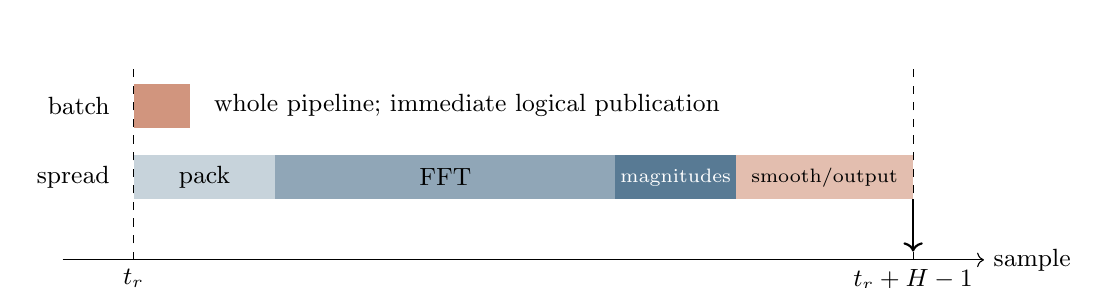
\begin{tikzpicture}[x=0.9cm,y=0.7cm,font=\small]
\draw[->] (0,0) -- (13,0) node[right]{sample};
\draw[dashed] (1,0) -- (1,3.5);
\draw[dashed] (12,0) -- (12,3.5);
\node[below] at (1,0) {$t_r$};
\node[below] at (12,0) {$t_r+H-1$};
\node[left] at (.8,2.8) {batch};
\fill[accent!65] (1,2.4) rectangle (1.8,3.2);
\node[right] at (2,2.8) {whole pipeline; immediate logical publication};
\node[left] at (.8,1.5) {spread};
\fill[ink!25] (1,1.1) rectangle (3,1.9);
\fill[ink!50] (3,1.1) rectangle (7.8,1.9);
\fill[ink!75] (7.8,1.1) rectangle (9.5,1.9);
\fill[accent!40] (9.5,1.1) rectangle (12,1.9);
\node at (2,1.5) {pack};
\node at (5.4,1.5) {FFT};
\node[font=\scriptsize,white] at (8.65,1.5) {magnitudes};
\node[font=\scriptsize] at (10.75,1.5) {smooth/output};
\draw[->,thick] (12,1.1) -- (12,.15);
\end{tikzpicture}
\caption{One selected frame, two placements of its complete analysis. The
spread path publishes only after the final logical credit. Stage widths are
schematic; credit balance does not imply equal execution time. Native hybrids
retain one indivisible FFT inside the distributed sequence.}
\label{fig:whole-timeline}
\end{figure}


The per-call bound covers scheduled window and cache rebuilds and the modules'
bounded output callbacks. Construction and host lifecycle callbacks are
excluded, and each call still performs constant input and control work plus an
$O(\log N)$ plan-index calculation. Because every stage is decomposed into
bounded operations, no $O(N)$ boundary pass remains in steady-state engine
analysis; the quota decides only where those operations run
(Figure~\ref{fig:whole-timeline}). Reweighting changes that placement, but it
cannot equalize operation costs, constrain an arbitrary user callback, or
bound operating-system interruptions.

\subsection{Retained samples, plans, and publication time}
Count continuously captured samples from zero and let the frame endpoint be
$t_r=rH$. The frame is selected on call $t_r$; its last credit and its
publication occur on call $t_r+H-1$. The last actual output may precede the
final credit, but it remains private until publication. The nominal
sample-index ages at publication are therefore
\begin{equation}
 A_{\mathrm{newest}}=(H-1)/f_s,\qquad
 A_{\mathrm{mid}}=((N-1)/2+H-1)/f_s.
 \label{eq:wholeage}
\end{equation}
These ages exclude elapsed computation and display delay. Successive
publications are exactly $H$ samples apart, in contrast to the original
scheduler's next-call publication in Equation~\eqref{eq:age}. At startup the
window is zero-padded rather than waiting for a full window of input. When the
hop changes, endpoints satisfy $t_{r+1}=t_r+H_r$, and each frame uses its
latched $H_r$.

Because packing is incremental, the selected samples must survive while
capture continues. A preallocated ring of capacity $C=N_{\max}+H_{\max}$
suffices for the prepared maximum window and hop, and no whole-frame copy of
the input is needed. Appendices~\ref{app:one-hop} and~\ref{app:implementation}
give the lifetime proof and the reuse of maximum-size tables.

\subsection{Smoothing, configuration, and output ownership}
Reconstruction computes magnitudes and, when frequency smoothing is enabled,
a prefix sum that is complete before any range average is emitted. Output then
applies an inclusive fractional-octave magnitude mean, optional temporal
averaging, and the module's display conversion. These are magnitude means, not
power means or a constant-Q analysis, and the window normalization and display
units are unchanged. Appendix~\ref{app:one-hop} records the equations, control
conventions, cache behavior, and the sample-level quantization of the hop.

Settings latch at the start of each frame, and a reset or sample-rate change
cancels any partial analysis. Window and smoothing caches rebuild inside
scheduled units, and a length change logically clears the input and averaging
history. Storage is prepared outside the sample path, with one exception:
increasing the supported hop in a sample-rate callback can allocate. Freeze
behaves differently in the two modules, so the continuous-input timestamp
formulas do not hold across a pause.

Each output bin is written to producer-owned storage. Only a complete frame is
published, through a single-producer/single-consumer triple-slot mailbox that
uses acquire/release atomic exchange. The consumer keeps its slot until its
next successful exchange, and the producer never writes to that slot, so a
slow consumer may miss intermediate snapshots but never reads a partially
written one. Fourier uses one curve mailbox; Spectre uses one mailbox per
history column and builds and recolors its image history on the UI thread.
Lifecycle work, other shared controls, UI work, and host scheduling lie
outside the quota, so the contract is not a general claim of hard real-time
safety.

\section{Experimental Method}
\label{sec:evaluation}
The study asks three questions. How much of a burst reduction comes from work
placement within a fixed implementation? How does that choice interact with
native kernels and the completion horizon? And does it improve
complete-module behavior under Rack's sample-synchronous engine? The questions
and the workload matrix were recorded before collection. The analysis is a
\emph{descriptive pilot study}: it reports what was observed and does not
select a winner and then confirm it.

\subsection{Host, sessions, and workload boundaries}
Two separately prepared sessions ran on September 30, 2026 (local time) on one
Apple M1 Pro laptop with macOS 26.6.2 and Apple Clang 21.0.0, using the same
executable and archived sources. The operator reported disconnecting
networking and Bluetooth and closing agents and unnecessary applications. The
runner required AC power with Low Power Mode off, held \code{caffeinate -is}
assertions, settled for 180 seconds after staging, and settled each fresh
process for one second before warmup. Snapshots taken before and after each
session confirm the power and sleep assertions. They also show residual macOS
service activity, including \code{sandboxd} and Spotlight indexing, and cannot
rule out interference during any particular interval.

Each session ran 194 planned cells twice, each time in a fresh process, for
776 processes in total. Three bridge cells repeat across groups, leaving 191
unique configurations. Group order was fixed, and process order within each
group followed predeclared session seeds. Every process and every slow
interval is retained. Table~\ref{tab:study-design} summarizes the seven
groups. Setup, plan creation, correctness replay, storage probes, and output
serialization all fall outside the timed block intervals.

\input{.build/paper-study/design.tex}

The stream harness times either complete analysis calls feeding a controlled
sink or the modules' actual \code{process()} paths, including input
conditioning and display-data conversion. Fourier's shipped defaults use four
SIMD lanes, $N=2048$, a 30\,ms hop ($H=1440$ at 48\,kHz), and a flattop
window; Spectre's use scalar samples, $N=2048$, $H=1024$, and a flattop
window. Unless stated otherwise, controlled scalar comparisons use a Hann
window, $H=1024$, no smoothing, and $D=64$. Every table and figure states
which boundary it measures.

The host group drives the pinned Rack engine's actual \code{stepBlock()},
including worker synchronization, with one or four engine threads; 0, 1, 4,
or 16 analyzers; and 0, 16, or 64 deterministic background modules. These form
a structured set of combinations rather than a full factorial design. Native
module controls replace only the analysis inside the same module shell,
keeping input conditioning, display conversion, and mailbox publication. They
also retain some unused production storage, so their footprint does not
represent the memory requirement of an optimized replacement. An optional
concurrent headless consumer copies and checksums snapshots at 30 or 60\,Hz,
with declared stalls; it neither draws a window nor drives an audio interface.

\subsection{Matched controls and native layouts}
The matched first-party batch and distributed controls share one scalar
analysis implementation, its arithmetic, and its storage, so they isolate
placement more cleanly than any comparison across FFT libraries. Each native
batch/hybrid pair likewise shares one retained-input, window, magnitude,
smoothing, and output path. Batch runs the whole sequence immediately; hybrid
distributes the surrounding stages but executes the transform and its
reordering as one indivisible native call. The native pipelines read
contiguous ring segments and use native output layouts, avoiding per-element
ring-modulo arithmetic and conversion to a canonical complex layout. vDSP
uses vectorized windowing and packing and batched four-channel transforms.
FFTW uses reusable real plans, including \code{plan\_many} for four channels,
created in each fresh process by single-threaded \code{FFTW\_MEASURE} planning
without imported wisdom. PFFFT uses its ordered packed spectrum. All paths
compute magnitudes with an explicitly scaled norm to avoid premature underflow
when squaring. These are strong native controls, but they do not exhaust every
provider-specific optimization.

The granularity group holds the frame hop fixed and varies the native
completion horizon over $H_c\in\{H,\ceil{H/2},\ceil{H/4}\}$. Publication
occurs at endpoint age $H_c-1$, after which the pipeline only captures input
until the next endpoint. This trades latency against the density of
surrounding-stage work without subdividing the native FFT. Native sub-FFT
leaves and new stage weights were deliberately deferred and have no measured
evidence here. The production weights, $p=4$ for window rebuilds and $o=2$
for Fourier output, were tuned in earlier engineering experiments on the same
M1 Pro, and band-cache rebuilding runs inside output units without additional
weight. The study therefore does not independently validate those weights.

\subsection{Timing, replication, and age}
Stream groups execute blocks back to back. The host group releases blocks on
an absolute periodic schedule with period $D/f_s$ and does not reset the
release origin after an overrun. A monotonic clock records wake, start, and
finish times separately. Threads inherit the default scheduling policy; no
core affinity, frequency lock, or real-time priority was applied. Stream
processes inherit and record their floating-point control state, while the
actual Rack engine applies its own per-block FPU policy. Empty-timer
observations are retained without subtraction, and reported values are
rounded to about three significant figures.

The primary burst statistic is the median \emph{per-hop peak block time}: for
each complete interval from one frame endpoint to the next, take the longest
duration of any whole block that intersects it. Unlike a callback percentile,
this statistic always captures a batch burst, however rare such bursts are
among all callbacks. A block that spans two hops counts toward both, and no
sub-block costs are imputed. Engine peaks use actual replay endpoints and the
full hop for both immediate and delayed publication. Lifecycle sequences are
excluded from this stationary statistic. Callback p99, maxima, and counts of
blocks exceeding $D/f_s$ are reported as secondary observations.

Stream cost is the sum of instrumented block wall times divided by the number
of engine samples. It therefore includes timer, dispatch, and interruption
effects; the design has no separate untimed throughput pass. Host results also
record process-wide user-plus-system CPU time over the measurement interval,
including workers, pacing overhead, and any headless consumer. CPU time and
block wall time are distinct quantities. A \emph{release miss} means that a
block finished after its synthetic release deadline, including wake lateness
and accumulated backlog. A \emph{compute-budget exceedance} means that the
timed block alone exceeded $D/f_s$. Neither is an audio-device underrun.

For each cell, costs are averaged over the two processes within a session,
and burst quantiles take the median of the two process summaries. Tables
report the midpoint of the two session summaries, their range where
indicated, and the largest retained observation. There are only two session
replicates, both on the same date and host, and callbacks, hops, analyzers,
and channels are dependent observations. We therefore report descriptive
variation rather than confidence intervals, rare-event probabilities, or
worst-case execution-time claims~\cite{kalibera2013,mytkowicz2009,wilhelm2008}.

Publication age is measured in logical engine samples from the frame
endpoint; center age adds $(N-1)/2$. Consumer age is bracketed by the
completed-block watermarks observed around each copy, leaving one block of
uncertainty. Final drains are excluded from ordinary consumer ages. These
sample-clock ages are not wall-clock freshness during an overrun, and they
exclude repaint.

\subsection{Numerical and provenance checks}
Every session passed checks of archive and artifact hashes, the exact
declared matrix and process order, execution sidecars, and a numerical replay
of every output. The independent references are direct DFTs at small lengths
and a separately structured binary64 FFT at larger lengths; module replays
also model DC conditioning and display conversion. Relative $\ell_2$ and
$\ell_\infty$ errors of each magnitude vector must not exceed
$3\times10^{-4}$ in float or $10^{-10}$ in double, and a zero reference
requires zero output. These are engineering acceptance budgets, not
guarantees for every weak bin.

A long complete-module decay fixture separately flags the region affected by
Rack's flush-to-zero behavior and Fourier's display mapping. It applies the
predeclared \code{module-decay-ftz-v1} absolute floor, retains every vector,
and excludes flagged vectors from relative-accuracy claims. The floor is an
engineering allowance, not a proven error bound. The distinction matters
because relative error can reach one in that tail while absolute error stays
below the floor. Native allocators are opaque to the separate C++ allocation
probe, so their storage and allocation calls are not observed.
Appendix~\ref{app:reproducibility} identifies the raw evidence and the
deterministic publication tools.

\section{Results}
\label{sec:comparison-results}
The measurements support three findings. Placement substantially changes the
typical burst of a fixed implementation. Native kernels change the cost of
obtaining that reduction. And complete host behavior depends on
synchronization, alignment, and release timing as well as on analyzer cost.

\subsection{Placement and native implementation cost}
Table~\ref{tab:study-baselines} reports the scalar reference shape. Matched
distribution reduces the median per-hop peak from \StudyBatchPeak{} to
\StudyCorePeak\,$\mu$s, a factor of \StudyPlacementRatio, while cost rises
from \StudyBatchCost{} to \StudyCoreCost\,ns per engine sample. Across all
three baseline lengths, all four matched implementation families, and both
sessions, the distributed or hybrid path has the lower session hop-peak
summary in \StudyPlacementSigns{} of \StudyPlacementComparisons{} comparisons.
This is descriptive sign consistency over dependent cells; it is neither a
significance test nor a ranking of unrelated kernels.

\input{.build/paper-study/baselines.tex}

Native kernels lower the price of a similar reduction. The PFFFT hybrid costs
\StudyPffftHybridCost\,ns/sample with an \StudyPffftHybridPeak\,$\mu$s hop
peak, against \StudyPffftBatchCost\,ns/sample and \StudyPffftBatchPeak\,$\mu$s
for its matched batch path; vDSP and FFTW supply further tradeoff points.
Figure~\ref{fig:study-tradeoff} shows every process at this shape. A small
peak does not imply minimal aggregate work, and the variation between sessions
is shown rather than folded into a single score per provider. Redistributing
work changes dispatch, vector-call sizes, and locality, so even matched
arithmetic need not produce identical elapsed cost.

\input{.build/paper-study/tradeoff.tex}

At this shape even the scalar batch path uses only a few percent of its
1,333\,$\mu$s block budget. The reference exists to isolate work placement;
its practical significance must be judged at the complete-module and host
boundaries below. Callback p99 and retained maxima also differ markedly from
the median hop peak: the per-hop statistic keeps sparse frame work visible,
whereas maxima retain interruptions and other excursions. None of these
statistics is a safe execution-time bound.

\subsection{Completion horizon and four-channel analysis}
The native horizon sweep makes publication age an explicit design variable
(Table~\ref{tab:study-horizons}). At the demanding controlled shape
$N=16384$, $H=240$, contracting the four-channel vDSP hybrid's horizon from
$H$ to $H/2$ to $H/4$ cuts endpoint age from 4.98 to 2.48 to 1.23\,ms while
raising its median hop peak from \StudyHorizonFullPeak{} to
\StudyHorizonHalfPeak{} to \StudyHorizonQuarterPeak\,$\mu$s. Because the
native FFT remains indivisible, a shorter horizon packs the surrounding stages
more densely without distributing the transform itself. Behavior at small
sizes and for other kernels need not be monotonic; all 39 granularity cells
are retained in the accompanying data.

\input{.build/paper-study/horizons.tex}

At the same four-channel shape, the SIMD production core has a
\StudySimdExtremePeak\,$\mu$s peak at \StudySimdExtremeCost\,ns/sample,
against \StudyHorizonFullPeak\,$\mu$s at \StudyHorizonFullCost\,ns/sample for
the full-hop vDSP hybrid. Here the native hybrid is better on both recorded
cost and typical peak. Channel-level SIMD therefore does not by itself give
the production core an advantage over batched native channels; which approach
wins depends on shape and kernel. These controlled rows omit module
conditioning and display conversion.

\subsection{Shipped defaults and demanding module settings}
Table~\ref{tab:study-modules} measures actual module calls with paced
releases. With its defaults, Fourier's hop peak is
\StudyModuleDefaultPeak\,$\mu$s, \StudyModuleDefaultBudgetPercent\% of the
block budget. At $N=16384$ with a 5\,ms hop, the complete four-port module
reaches \StudyModuleExtremePeak\,$\mu$s, or
\StudyModuleExtremeBudgetPercent\%. Enabling both smoothing modes raises this
to \StudyModuleBothPeak\,$\mu$s (\StudyModuleBothBudgetPercent\%), with
\StudyModuleBothComputeMisses{} compute-budget exceedances and
\StudyModuleBothMisses{} late releases in 3,840 blocks. The hardest shipped
setting is thus a materially different regime from both the scalar reference
and the defaults.

\input{.build/paper-study/modules.tex}

Using one active port does not make Fourier a scalar analyzer: its four-lane
analysis still runs, and additional voices are summed into each port's lane
rather than becoming separate FFT channels. The table therefore captures
control and input costs and does not imply a fourfold saving when three ports
are unpatched. No paced native complete-module comparison was collected at the
extreme shape, and the continuous native core results cannot fill that gap.
These settings expose a limitation of the production path; they are not
evidence that an alternative would eliminate its missed releases.

\subsection{Actual Rack engine, alignment, and missed releases}
Four aligned Fourier modules on one engine thread produce a large difference
in concentration (Table~\ref{tab:study-host}). Production's typical hop peak
of \StudyHostCorePeak\,$\mu$s uses \StudyHostCoreBudgetPercent\% of the
budget, against \StudyHostBatchPeak\,$\mu$s (\StudyHostBatchBudgetPercent\%)
for vDSP batch and \StudyHostHybridPeak\,$\mu$s
(\StudyHostHybridBudgetPercent\%) for the vDSP hybrid. The price is aggregate
block wall cost: \StudyHostCoreCost{} versus \StudyHostBatchCost{} and
\StudyHostHybridCost\,ns/sample, respectively. In this regime the burst
reduction frees a substantial fraction of the block for other work, rather
than shaving a few microseconds from an otherwise idle callback.

\input{.build/paper-study/host.tex}

Four engine threads change the picture. With four aligned modules, the three
paths converge to typical hop peaks of 100--115\,$\mu$s
(Figure~\ref{fig:study-host}), and the empty four-thread engine has a much
larger callback p99 than the one-thread control. Rack's per-sample barriers
and worker dispatch are a plausible mechanism, but these runs do not separate
that cost from CPU placement or power-state effects, and the synchronization
code alone does not establish it. Table~\ref{tab:study-host-accounting} adds
an important observation: the empty four-thread engine consumes about
\StudyEmptyCpuCores{} CPU-seconds per second of nominal audio, consistent with
workers spinning between releases, and its process CPU stays near that level
when analyzers are present. The one-thread engine, by contrast, can sleep
between releases. Moving to four threads therefore changes the activity and
potential power-state regime as well as the available parallelism. We report
this as the observed behavior of the pinned headless engine, not as an
isolated measurement of barrier overhead.

\input{.build/paper-study/host-accounting.tex}

\input{.build/paper-study/host-figure.tex}

With 16 aligned modules on four threads, production's typical peak is
\StudyHostManyCorePeak\,$\mu$s against \StudyHostManyBatchPeak\,$\mu$s for
vDSP batch, and staggering the native instances lowers the batch peak to
\StudyHostStaggerBatchPeak\,$\mu$s. Staggering is thus a practical
alternative whenever frame phases can be chosen. The predeclared sweep of 0,
16, and 64 background modules with four staggered analyzers did not reach a
repeatable saturation point, and its latency summaries are not monotonic in
the number of background modules. We retain those cells but do not treat the
background-module count as a calibrated CPU load.

Release misses call for a stronger qualification. On one thread with four
modules, production and vDSP batch have \StudyHostCoreMisses{} and
\StudyHostBatchMisses{} late releases despite very different typical peaks,
and the vDSP hybrid has \StudyHostHybridMisses. The corresponding FFTW batch
row has \StudyHostFftwBatchMisses, but that provider-specific outcome does not
demonstrate a general benefit of scheduling. With 16 aligned modules,
production has \StudyHostManyCoreMisses{} late releases while vDSP batch has
none in these runs, and even empty-engine controls miss releases. These counts
are observations under synthetic pacing and include wake delay and backlog.
They support comparisons of headroom and concentration; they do not establish
fewer audio underruns or a stable ordering of rare-event reliability.

\subsection{Consumer age and numerical limits}
Table~\ref{tab:study-consumer} reports the headless consumer. At 60\,Hz,
production and the full-hop vDSP hybrid have median endpoint-age bounds of
38--40\,ms, against 8--10\,ms for native batch. The difference, about one
30\,ms hop, matches the publication contract. At 30\,Hz, or with polling
stalls, some complete Fourier snapshots are superseded before they are read:
correct ownership protects the data a consumer holds, but it does not
guarantee that the consumer sees every frame. Logical age bounds do not
measure screen refresh, perceptual acceptability, or real-time freshness
during a backlog.

\input{.build/paper-study/consumer.tex}

All numerical replays pass their declared policies
(Table~\ref{tab:study-numerical}), including non-power-of-two hops, high
overlap, weak and decaying input, silence, and complete-module lifecycle
changes. Preparing the study exposed premature underflow in naively squared
magnitudes, and the measured source uses scaled magnitudes in both production
and native paths. Long decays still reach the flagged FTZ/display tail, where
observed relative error can reach one, so the ordinary relative budgets do not
extend to that region. Retaining the tail with its absolute diagnostics is
more informative than labeling the entire decay uniformly accurate.

\input{.build/paper-study/numerical.tex}

Lifecycle replays check freeze and resume, window and band changes, geometry
changes, reset, and sample-rate changes separately from the stationary
comparisons. These mutations occur between engine blocks, and their durations
and allocation probes are recorded outside ordinary block intervals. The study
thus verifies serialized lifecycle behavior; it does not show that arbitrary
concurrent control changes, or all host callbacks, are allocation-free.

\FloatBarrier
\section{Discussion and Limits}
\label{sec:discussion}
\subsection{Choosing execution granularity}
The results suggest a practical procedure. Start with native batch execution
under the required complete-path semantics: if its per-hop peaks fit the
analysis budget and fresh output matters, immediate execution is a strong
choice. If aligned releases consume too much headroom, try staggering or a
native hybrid, and shorten the hybrid's horizon when age matters. Choose
butterfly-level scheduling when its measured complete-path behavior meets a
requirement that the coarser alternatives do not, at an acceptable total cost.

This is an empirical design rule, not a deadline guarantee. The four-module,
one-thread result is the clearest practical case: relative to vDSP batch, the
production path reduces typical block concentration from about two-thirds of
the budget to about 15\%. Yet the native hybrid is competitive in several
controlled shapes, and the multithreaded engine changes the ranking. The
execution contract remains useful across all of these choices, but
performance cannot be inferred from the number of resumable butterflies alone.
Because Rack's CPU meter reflects aggregate cost, a path with smaller bursts
can still appear more expensive to a user.

Publication age is an explicit cost. A 30\,ms hop adds about 1.8 frames of a
60\,Hz display before polling and repaint, although that arithmetic does not
establish a perceptual threshold. For latest-frame visualization, a UI or
worker thread may be preferable; for exact-hop producer history, such a design
must specify its capture, queueing, overflow, and ownership policy. Spectre's
history storage and per-column mailboxes serve a different consumer contract
from Fourier's latest curve. These alternatives deserve measurement at
equivalent boundaries before broader recommendations are made.

\subsection{What the evidence can establish}
Native layouts, actual module and engine processing, and a concurrent consumer
connect the controlled analyzer to its host. Both pilots, however, used one
M1 Pro, one binary, one compiler, and one date. This is an early Apple Silicon
laptop, neither the base M1 nor a lower performance bound for Apple hardware.
Replication on independent days, with independent builds, and on other
architectures remains outstanding.

Careful setup and power and sleep checks coexist with residual OS activity.
Snapshots cannot identify the cause of an individual outlier; longer compute
paths may be more exposed to interruption, but that mechanism was not
isolated. Maxima and session ranges retain those observations. The fixed group
order also confounds workload family with time and possible thermal drift.

The stream study lacks a separate throughput pass, a matched comparison of
paced and continuous execution at identical boundaries, core-placement
calibration, and a thread-policy sweep. Because four-thread engine workers
consume substantial CPU even in an empty graph, changes with thread count
cannot be attributed to parallel analysis alone. The background sweep did not
locate a saturation threshold, and the extreme module settings lack matched
paced native controls. These gaps limit causal and reliability claims, even
though every reported comparison is traceable to retained data. Headless
consumption verifies copying, ownership, and logical age; device underruns,
GUI load, and repaint are outside its scope. Native allocator internals remain
opaque, and the unused module storage retained by the native controls
precludes a ranking by total memory.

\subsection{Scope of the contribution}
The analytical result bounds credits for a complete dependency-ordered
analyzer. The conditional operation-cost bound explains how weights could be
chosen, whereas the measurements test implementations on one host; cache
effects, unequal unit costs, interrupts, and unrelated engine work separate
these two claims. The empirically tuned weights and the unweighted band-cache
rebuild are implementation choices, not a proof of time balance.

Time-distributed transforms and cooperative processing chains precede this
work. The specific contribution is to combine analysis-tail accounting,
exact-hop cadence, input lifetime, cancellation, and output ownership in one
contract, and to evaluate it with comparisons that expose placement, kernel,
and host effects. Native sub-FFT leaves could improve the tradeoff and remain
the most important unmeasured granularity. Inverse synthesis and long-filter
convolution need their own bounded preparation and delivery stages, and this
analysis-only study makes no performance claim for them.

\section{Conclusion}
Complete windowed analysis can advance over an exact hop as one bounded
sequence covering preparation, transform, magnitude processing, smoothing, and
publication. Whole-pipeline accounting removes the boundary bursts and cadence
error of FFT-only scheduling, while input retention and mailbox ownership
protect the analyzed samples and the published spectra.

A descriptive study separates this contract from implementation cost. Matched
scheduling reduces typical hop peaks, and native hybrids and shorter
completion horizons offer different tradeoffs between cost and age. With four
aligned Rack modules on one engine thread, the production pipeline
substantially reduces block concentration relative to native batch execution.
Synchronization, staggering, and release lateness nevertheless reshape
host-level outcomes, and missed releases give no consistent reliability
ranking. Execution granularity should therefore be chosen against measured
complete-path headroom and age requirements; broader platform and
audio-device claims require further measurement.

\clearpage
\begin{thebibliography}{99}
\small\raggedright
\bibitem{cooley1965}
J. W. Cooley and J. W. Tukey, ``An algorithm for the machine calculation of
complex Fourier series,'' \emph{Mathematics of Computation}, vol. 19, no. 90,
pp. 297--301, 1965. \href{https://doi.org/10.1090/S0025-5718-1965-0178586-1}{doi:10.1090/S0025-5718-1965-0178586-1}.

\bibitem{sorensen1987}
H. V. Sorensen, D. L. Jones, M. T. Heideman, and C. S. Burrus,
``Real-valued fast Fourier transform algorithms,'' \emph{IEEE Transactions
on Acoustics, Speech, and Signal Processing}, vol. 35, no. 6, pp. 849--863,
1987. \href{https://doi.org/10.1109/TASSP.1987.1165220}{doi:10.1109/TASSP.1987.1165220}.

\bibitem{allen1977}
J. B. Allen and L. R. Rabiner, ``A unified approach to short-time Fourier
analysis and synthesis,'' \emph{Proceedings of the IEEE}, vol. 65, no. 11,
pp. 1558--1564, 1977.
\href{https://doi.org/10.1109/PROC.1977.10770}{doi:10.1109/PROC.1977.10770}.

\bibitem{harris1978}
F. J. Harris, ``On the use of windows for harmonic analysis with the discrete
Fourier transform,'' \emph{Proceedings of the IEEE}, vol. 66, no. 1,
pp. 51--83, 1978.
\href{https://doi.org/10.1109/PROC.1978.10837}{doi:10.1109/PROC.1978.10837}.

\bibitem{lo1998}
P.-C. Lo and Y.-Y. Lee, ``Real-time implementation of the split-radix FFT---an
algorithm to efficiently construct local butterfly modules,''
\emph{Signal Processing}, vol. 71, no. 3, pp. 291--299, 1998.
\href{https://doi.org/10.1016/S0165-1684(98)00152-2}{doi:10.1016/S0165-1684(98)00152-2}.

\bibitem{lo1999}
P.-C. Lo and Y.-Y. Lee, ``Real-time FFT algorithm applied to on-line spectral
analysis,'' \emph{Circuits, Systems, and Signal Processing}, vol. 18, no. 4,
pp. 377--393, 1999.
\href{https://doi.org/10.1007/BF01200789}{doi:10.1007/BF01200789}.

\bibitem{lomoving1999}
P.-C. Lo and Y.-Y. Lee, ``Real-time implementation of the moving FFT
algorithm,'' \emph{Signal Processing}, vol. 79, no. 3, pp. 251--259, 1999.
\href{https://doi.org/10.1016/S0165-1684(99)00098-5}{doi:10.1016/S0165-1684(99)00098-5}.

\bibitem{borss2009}
C. Bor\ss{}, ``A VST reverberation effect plugin based on synthetic room
impulse responses,'' in \emph{Proceedings of the 12th International Conference
on Digital Audio Effects (DAFx-09)}, Como, Italy, September 2009.
\url{https://www.dafx.de/paper-archive/2009/papers/paper_48.pdf}.

\bibitem{hurchalla2010}
J. Hurchalla, ``A time distributed FFT for efficient low latency convolution,''
in \emph{129th Audio Engineering Society Convention}, paper 8257, 2010.
\url{https://secure.aes.org/forum/pubs/conventions/?elib=15679}.

\bibitem{battenberg2011}
E. Battenberg and R. Avi\v{z}ienis, ``Implementing real-time partitioned
convolution algorithms on conventional operating systems,'' in
\emph{Proceedings of the 14th International Conference on Digital Audio
Effects (DAFx-11)}, Paris, France, September 2011.
\url{https://ericbattenberg.com/pdf/partconvDAFx2011.pdf}.

\bibitem{wefers2015}
F. Wefers, \emph{Partitioned Convolution Algorithms for Real-Time Auralization},
Aachener Beitr\"age zur Technischen Akustik, vol. 20. Berlin: Logos Verlag, 2015.
Ph.D. dissertation, RWTH Aachen University, defended 2014.
\href{https://doi.org/10.18154/RWTH-2015-02185}{doi:10.18154/RWTH-2015-02185}.

\bibitem{liu2017}
J. Liu, B. Yan, and Q. Zou, ``Optimal time-distributed fast Fourier transform:
Application to online iterative learning control---experimental high-speed
nanopositioning example,'' \emph{Mechatronics}, vol. 41, pp. 114--124, 2017.
\href{https://doi.org/10.1016/j.mechatronics.2016.11.007}{doi:10.1016/j.mechatronics.2016.11.007}.

\bibitem{prusa2016}
Z. Pr\r{u}\v{s}a and N. Holighaus, ``Real-time audio visualization with
reassigned non-uniform filter banks,'' in \emph{Proceedings of the 19th
International Conference on Digital Audio Effects (DAFx-16)}, Brno,
Czech Republic, pp. 3--8, September 2016.
\url{https://www.dafx.de/paper-archive/2016/dafxpapers/01-DAFx-16_paper_20-PN.pdf}.

\bibitem{jacobsen2003}
E. Jacobsen and R. Lyons, ``The sliding DFT,'' \emph{IEEE Signal Processing
Magazine}, vol. 20, no. 2, pp. 74--80, 2003.
\href{https://doi.org/10.1109/MSP.2003.1184347}{doi:10.1109/MSP.2003.1184347}.

\bibitem{lyons2021}
R. Lyons and C. Howard, ``Improvements to the sliding discrete Fourier
transform algorithm,'' \emph{IEEE Signal Processing Magazine}, vol. 38,
no. 4, pp. 119--127, 2021.
\href{https://doi.org/10.1109/MSP.2021.3075416}{doi:10.1109/MSP.2021.3075416}.

\bibitem{richardson2019}
L. F. Richardson and W. F. Eddy, ``Algorithm 991: The 2D tree sliding window
discrete Fourier transform,'' \emph{ACM Transactions on Mathematical Software},
vol. 45, no. 1, article 12, 2019.
\href{https://doi.org/10.1145/3264426}{doi:10.1145/3264426}.
Preprint: \url{https://arxiv.org/abs/1707.08213}.

\bibitem{garrido2016}
M. Garrido, ``The feedforward short-time Fourier transform,''
\emph{IEEE Transactions on Circuits and Systems II: Express Briefs},
vol. 63, no. 9, pp. 868--872, 2016.
\href{https://doi.org/10.1109/TCSII.2016.2534838}{doi:10.1109/TCSII.2016.2534838}.

\bibitem{park2014}
C.-S. Park and S.-J. Ko, ``The hopping discrete Fourier transform,''
\emph{IEEE Signal Processing Magazine}, vol. 31, no. 2, pp. 135--139, 2014.
\href{https://doi.org/10.1109/MSP.2013.2292891}{doi:10.1109/MSP.2013.2292891}.

\bibitem{rafii2018}
Z. Rafii, ``Sliding discrete Fourier transform with kernel windowing,''
\emph{IEEE Signal Processing Magazine}, vol. 35, no. 6, pp. 88--92, 2018.
\href{https://doi.org/10.1109/MSP.2018.2855727}{doi:10.1109/MSP.2018.2855727}.

\bibitem{eleftheriadis2023}
C. Eleftheriadis, M. Garrido, and G. Karakonstantis, ``Energy-efficient
short-time Fourier transform for partial window overlapping,'' in
\emph{Proceedings of the IEEE International Symposium on Circuits and
Systems (ISCAS)}, 2023.
\href{https://doi.org/10.1109/ISCAS46773.2023.10181940}{doi:10.1109/ISCAS46773.2023.10181940}.

\bibitem{becoulet2021}
A. B\'ecoulet and A. Verguet, ``A depth-first iterative algorithm for the
conjugate pair fast Fourier transform,'' \emph{IEEE Transactions on Signal
Processing}, vol. 69, pp. 1537--1547, 2021.
\href{https://doi.org/10.1109/TSP.2021.3060279}{doi:10.1109/TSP.2021.3060279}.

\bibitem{frigo2005}
M. Frigo and S. G. Johnson, ``The design and implementation of FFTW3,''
\emph{Proceedings of the IEEE}, vol. 93, no. 2, pp. 216--231, 2005.
\href{https://doi.org/10.1109/JPROC.2004.840301}{doi:10.1109/JPROC.2004.840301}.
Planner API: \url{https://www.fftw.org/fftw3_doc/Planner-Flags.html}
(accessed September 30, 2026).

\bibitem{pffft}
J. Pommier and contributors, ``PFFFT: A pretty fast FFT,'' software;
VCV Rack integration, \code{dsp::RealFFT}. Accessed September 30, 2026.
\url{https://github.com/VCVRack/pffft}.
\href{https://github.com/VCVRack/Rack/blob/v2/include/dsp/fft.hpp}{Rack FFT wrapper source}.

\bibitem{vdsp}
Apple, ``Using Fourier Transforms,''
\href{https://developer.apple.com/library/archive/documentation/Performance/Conceptual/vDSP_Programming_Guide/UsingFourierTransforms/UsingFourierTransforms.html}{\emph{vDSP Programming Guide}},
Accelerate framework documentation. Accessed September 30, 2026.

\bibitem{vanderbyl2016}
A. van der Byl and M. R. Inggs, ``Constraining error---a sliding discrete
Fourier transform investigation,'' \emph{Digital Signal Processing},
vol. 51, pp. 54--61, 2016.
\href{https://doi.org/10.1016/j.dsp.2016.01.008}{doi:10.1016/j.dsp.2016.01.008}.

\bibitem{skare2024}
T. Skare, ``General-purpose GPU audio benchmark framework,'' in
\emph{Proceedings of the 27th International Conference on Digital Audio
Effects (DAFx24)}, Guildford, United Kingdom, pp. 452--458, September 2024.
\url{https://www.dafx.de/paper-archive/2024/papers/DAFx24_paper_56.pdf}.

\bibitem{balasubramaniam2026}
D. R. K. Balasubramaniam, S. Ramachandran, and J. Timoney,
``Real-time neural audio on Apple Silicon: Benchmarking inference frameworks
under realistic DAW contention,'' in \emph{Proceedings of the 29th
International Conference on Digital Audio Effects (DAFx26)}, Cambridge, MA,
USA, pp. 128--135, September 2026.
\url{https://www.dafx.de/paper-archive/2026/papers/DAFx26_paper_16.pdf}.

\bibitem{mytkowicz2009}
T. Mytkowicz, A. Diwan, M. Hauswirth, and P. F. Sweeney,
``Producing wrong data without doing anything obviously wrong!,'' in
\emph{Proceedings of the 14th International Conference on Architectural
Support for Programming Languages and Operating Systems (ASPLOS '09)},
pp. 265--276, 2009.
\href{https://doi.org/10.1145/1508244.1508275}{doi:10.1145/1508244.1508275}.

\bibitem{kalibera2013}
T. Kalibera and R. Jones, ``Rigorous benchmarking in reasonable time,'' in
\emph{Proceedings of the 2013 International Symposium on Memory Management
(ISMM '13)}, pp. 63--74, 2013.
\href{https://doi.org/10.1145/2464157.2464160}{doi:10.1145/2464157.2464160}.
Corrected author manuscript: \url{https://kar.kent.ac.uk/33611/}.

\bibitem{wilhelm2008}
R. Wilhelm et al., ``The worst-case execution-time problem---overview of
methods and survey of tools,'' \emph{ACM Transactions on Embedded Computing
Systems}, vol. 7, no. 3, article 36, 53 pages, 2008.
\href{https://doi.org/10.1145/1347375.1347389}{doi:10.1145/1347375.1347389}.

\bibitem{rack}
VCV, ``Plugin API guide,'' \emph{VCV Rack Manual}. Accessed September 28, 2026.
\url{https://vcvrack.com/manual/PluginGuide}.
\bibitem{gardner1995}
W. G. Gardner, ``Efficient convolution without input-output delay,''
\emph{Journal of the Audio Engineering Society}, vol. 43, no. 3,
pp. 127--136, March 1995.
\url{https://secure.aes.org/forum/pubs/journal/?elib=7957}.

\bibitem{garcia2002}
G. Garcia, ``Optimal filter partition for efficient convolution with short
input/output delay,'' \emph{113th Audio Engineering Society Convention},
paper 5660, October 2002.
\url{https://secure.aes.org/forum/pubs/conventions/?elib=11275}.

\bibitem{wefers2011}
F. Wefers and M. Vorl\"ander, ``Optimal filter partitions for real-time FIR
filtering using uniformly-partitioned FFT-based convolution in the
frequency-domain,'' in \emph{Proceedings of DAFx-11}, Paris, France,
pp. 155--161, 2011.
\url{https://www.dafx.de/paper-archive/2011/Papers/74_e.pdf}.

\bibitem{rackengine}
VCV, ``Rack engine implementation,'' source revision
\code{8c33d966d329e4a6e354593b2b5f9ac2df5a03bd}, inspected September 30, 2026.
\url{https://github.com/VCVRack/Rack/blob/8c33d966d329e4a6e354593b2b5f9ac2df5a03bd/src/engine/Engine.cpp}.

\end{thebibliography}

\clearpage
\appendix
\section{Transform Derivations and Resumable Traversal}
\label{sec:legacy-transform}
The frame and normalization convention is defined in
Section~\ref{sec:signal-model}. This appendix records the conventional
transform mathematics and the original state transition used by the reusable
FFT classes; the complete analysis schedule is in Section~\ref{sec:one-hop}.

\subsection{Resumable complex transform}
For $N=2^p$, bit reversal places the input in the order required by an iterative
radix-2 decimation-in-time transform. A stage of span $s=2,4,\ldots,N$ visits
groups $g=0,s,2s,\ldots,N-s$ and pairs $a=0,\ldots,s/2-1$. One step computes
\begin{align}
 e&=c[g+a], & o&=W_N^{aN/s}c[g+a+s/2],\\
 c[g+a]&\leftarrow e+o, & c[g+a+s/2]&\leftarrow e-o,
 \label{eq:butterfly}
\end{align}
where $W_N=\exp(-j2\pi/N)$. Advancing $a$, then $g$, then $s$ defines a serial
traversal of the conventional FFT graph. Retaining these three indices is
sufficient to suspend and resume that traversal. Each stage has $N/2$
butterflies, so the total count is
\begin{equation}
 B_c(N)=\frac{N}{2}\log_2 N.
 \label{eq:countcomplex}
\end{equation}
The coefficient array, twiddle table, and bit-reversal table each occupy
$O(N)$ storage; the traversal state occupies $O(1)$ storage. Buffer preparation
copies and permutes the entire frame. Resumability applies to the subsequent
butterfly traversal, not automatically to that preparation.

\begin{proposition}[Arithmetic-order preservation]
For a fixed buffered frame and transform configuration, any partition of the
serial butterfly traversal into finite batches yields the same completed
coefficient array as uninterrupted traversal, provided every butterfly executes
exactly once in the original order and no external code mutates the state.
\end{proposition}
\begin{proof}
After buffering, the two traversals have identical coefficients and indices.
If they agree before a butterfly, Equation~\eqref{eq:butterfly} reads the same
operands and performs the same updates; the index transition also agrees.
Induction over $B_c$ establishes equality. A pause changes no state. In floating
point, bitwise equality additionally assumes the same arithmetic instructions,
rounding environment, and compiler transformations; we assert it only within
a single executable, not across compilers or FFT libraries.
\end{proof}

\begin{lstlisting}[float=tbp,language=C++,caption={Simplified state transition corresponding to the original complex FFT. Tables and storage are prepared separately.},label={lst:step}]
void step() {
    if (span > N) return;
    const size_t half = span / 2;
    const auto even = c[group + pair];
    const auto odd = multiply(c[group + pair + half],
                              twiddle[pair * (N / span)]);
    c[group + pair] = even + odd;
    c[group + pair + half] = even - odd;
    if (++pair == half) {
        pair = 0;
        group += span;
        if (group == N) { group = 0; span *= 2; }
    }
}
\end{lstlisting}

\subsection{Real-input packing and reconstruction}
For even $N$, define $M=N/2$ and pack
$z[m]=u[2m]+j u[2m+1]$. Let $Z$ be its $M$-point complex transform.
For $1\le k<M$, with
$A=Z[k]$ and $D=\overline{Z[M-k]}$, reconstruction is
\begin{equation}
 X[k]=\frac{1}{2}\bigl(A+D-jW_N^k(A-D)\bigr),\qquad
 X[N-k]=\overline{X[k]}.
 \label{eq:real}
\end{equation}
The endpoints are
$X[0]=\Re Z[0]+\Im Z[0]$ and
$X[M]=\Re Z[0]-\Im Z[0]$.
This follows by separating the transforms of the even and odd real samples;
it is a standard consequence of conjugate symmetry, not a new real FFT.

The resumable inner transform performs
\begin{equation}
 B_r(N)=B_c(N/2)=\frac{N}{4}\log_2(N/2)
 \label{eq:countreal}
\end{equation}
butterflies. The original real-FFT class materializes all $N$ output bins, including conjugate
copies, and reconstructs them in one $O(N)$ loop when the last inner butterfly
finishes. Thus a real-FFT \code{step()} is not uniformly a single butterfly:
the completing step also performs reconstruction. The operational distinction
is essential to the timing model in Appendix~\ref{sec:cost}.

The inverse class uses
$\operatorname{IFFT}(X)=\overline{\operatorname{FFT}(\overline X)}/N$.
It treats each output normalization as an additional resumable step, giving
$B_c(N)+N$ steps after buffering. This differs from the real forward transform's
bulk reconstruction. Input copying, permutation, and conjugation remain
$O(N)$ buffering work. Neither production visualization module uses the
inverse transform. Applications of it need their own normalization,
buffering, and delivery contracts and are outside this analysis-only study.

\section{Original Scheduling, Cadence, and Latency}
\label{sec:scheduling}
Let $H\ge1$ be the requested computation horizon in sample calls and let $B>0$
be the number of inner butterflies. The implementation chooses
\begin{equation}
 q=\ceil{B/H}
 \label{eq:quota}
\end{equation}
and invokes the single-step method $q$ times per call. Once complete, further
step invocations are no-ops. The following statements concern this integer
model. The reusable forward classes compute the ceiling through
single-precision floating-point division; the repository's verification
checks the model over its tested range. Extremely large sizes or horizons require a separate analysis of
rounding and integer overflow. Zero horizons and unsupported transform lengths
are outside the forward-path contract examined here. We use powers of two
$N\ge4$ for the real transform.

\begin{proposition}[Completion bound]
The transform completes after exactly $L=\ceil{B/q}$ calls, with $L\le H$.
\end{proposition}
\begin{proof}
After $\ell$ calls the number of completed butterflies is
$\min(B,\ell q)$. The least $\ell$ reaching $B$ is $\ceil{B/q}$.
Since $qH\ge B$, this value cannot exceed $H$.
\end{proof}

This is a bound on operation counts, not execution time. In particular,
completion \emph{within} $H$ calls does not imply completion \emph{at} call $H$.
In the original snapshot, both visualization modules test completion at the start of their processing
routine, publish the previous result, buffer a new frame, and then advance the
new transform. In steady state, with constant parameters and active processing,
frame starts are therefore separated by $L$ samples rather than necessarily by
$H$ samples. Initialization, freeze, reset, and reconfiguration are separate
state transitions and are not covered by this steady-state statement.

\begin{table}[tb]
\centering
\begin{tabular}{@{}rrrrrr@{}}
\toprule
$N$ & $H=N/2$ & $B_r$ & $q$ & $L$ & $H/L$ \\
\midrule
1,024 & 512 & 2,304 & 5 & 461 & 1.111 \\
2,048 & 1,024 & 5,120 & 5 & 1,024 & 1.000 \\
4,096 & 2,048 & 11,264 & 6 & 1,878 & 1.091 \\
16,384 & 8,192 & 53,248 & 7 & 7,607 & 1.077 \\
\bottomrule
\end{tabular}
\caption{Derived real-FFT schedules. $H/L$ is the actual frame rate divided by the nominal rate when a new frame starts immediately after completion. These are operation counts, not timing measurements.}
\label{tab:cadence}
\end{table}


For $N=4096$ and $H=2048$, $q=6$ and $L=1878$. At 48 kHz the nominal
interval is 42.67 ms, whereas the original steady-state interval is
39.125 ms. The rate difference is about 9.1\%. This is not a numerical FFT
error; it is a difference between the parameter's nominal interpretation and
the scheduler's completion-driven frame clock.

\subsection{Timestamp semantics}
Suppose a complete input window is captured on call $t_r$ and its first batch
runs in that same call. Its final batch runs at $t_r+L-1$, and the module
publishes the result at the start of call $t_r+L$. Measured from the newest
sample, publication delay is consequently $L/f_s$. Relative to the midpoint
of the captured sample support, its age is
\begin{equation}
 A_{\mathrm{mid}}=\frac{(N-1)/2+L}{f_s}.
 \label{eq:age}
\end{equation}
The midpoint is a timestamp convention, not a universal group-delay claim for
arbitrary windows. The display thread may add further delay. Figure~\ref{fig:timeline}
separates the sample support from the deferred calculation. Streaming input
continues during calculation, but those newer samples belong to a later frame.

\begin{figure}[tb]
\centering
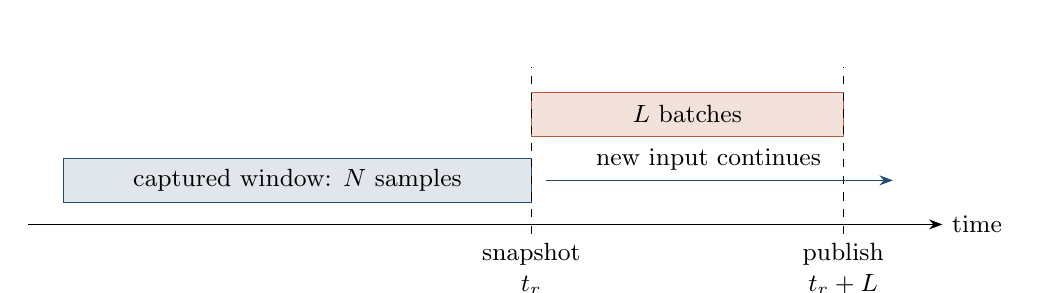
\begin{tikzpicture}[x=0.9cm,y=0.8cm,>=Stealth,font=\small]
\draw[->] (0,0)--(12.9,0) node[right] {time};
\fill[ink!14] (0.5,0.35) rectangle (7.1,1.05);
\draw[ink] (0.5,0.35) rectangle (7.1,1.05);
\node at (3.8,0.7) {captured window: $N$ samples};
\fill[accent!18] (7.1,1.4) rectangle (11.5,2.1);
\draw[accent] (7.1,1.4) rectangle (11.5,2.1);
\node at (9.3,1.75) {$L$ batches};
\draw[dashed] (7.1,-0.15)--(7.1,2.5);
\draw[dashed] (11.5,-0.15)--(11.5,2.5);
\node[below,align=center] at (7.1,-0.15) {snapshot\\$t_r$};
\node[below,align=center] at (11.5,-0.15) {publish\\$t_r+L$};
\draw[->,ink] (7.3,0.7)--(12.2,0.7);
\node[above] at (9.6,0.7) {new input continues};
\end{tikzpicture}
\caption{Logical timeline, not to scale. The transform operates on an owned copy of the captured frame while the input ring continues to advance. A smaller batch quota delays publication without changing that frame's spectral contents.}
\label{fig:timeline}
\end{figure}


\subsection{Consequences for temporal smoothing}
The original modules use an exponential magnitude smoother. Writing its intended time
constant as $\tau$ and assuming a nominal interval $H/f_s$ gives
\begin{equation}
 y_r=\alpha y_{r-1}+(1-\alpha)|X_r|,\qquad
 \alpha=\exp[-H/(f_s\tau)].
\end{equation}
The implementation's user-facing smoothing-time parameter corresponds to
$10\tau$. If actual updates arrive every $L/f_s$, then after elapsed time $t$
the old state is attenuated approximately by
$\exp[-tH/(L\tau)]$. The effective time constant is thus
\begin{equation}
 \tau_{\mathrm{eff}}=\tau L/H.
\end{equation}
For the 4096-point example, the decay time is approximately 8.3\% shorter than
its nominal interpretation. The one-hop successor removes this
completion-driven discrepancy, although the Fourier module still truncates its
hop control to integer samples (Section~\ref{sec:one-hop}). The analysis also
motivates timestamping
spectrogram columns by captured frames rather than assuming the configured
horizon is their spacing.

\subsection{Exact-horizon alternative}
If an application requires publication exactly every $H$ calls, it can separate
the frame clock from completion and retain a finished result until its scheduled
publication. Alternatively, apply Equation~\eqref{eq:balanced} to the $B$
ordered butterfly units in place of the complete pipeline's $W$ units.
The quotas sum to $B$ by telescoping; each is either $\floor{B/H}$ or
$\ceil{B/H}$. For $B>0$, the last quota is positive, so the ordered work ends
on call $H$. Among schedules for $B$ unit-cost operations in $H$ calls, no
schedule can have a maximum quota smaller than $\ceil{B/H}$, by the pigeonhole
principle. Equation~\eqref{eq:balanced} attains that lower bound. This elementary
balanced schedule is not a claimed new scheduling result. The successor applies
it to a larger work sequence (Section~\ref{sec:one-hop}). Its unit-cost premise
does not make unequal operations interchangeable in execution time.

\section{Original Whole-Pipeline Cost and Ownership}
\label{sec:cost}
The real FFT's public interface exposes a useful but partial work budget.
A schematic call-cost model is
\begin{equation}
 C_s=C_{\mathrm{input},s}+C_{\mathrm{dispatch},s}
       +b_s C_{\mathrm{butterfly},s}
       +\mathbf{1}_{s=0}C_{\mathrm{prepare}}
       +\mathbf{1}_{s=L-1}C_{\mathrm{reconstruct}}
       +C_{\mathrm{publish},s}.
 \label{eq:cost}
\end{equation}
Here $b_s\le q$ is the number of useful butterflies, and costs need not be
constant across stages or calls. Publication of a previous result may coincide
with preparation of the next. The expression describes locations of work,
not a hardware-independent cycle prediction.

In the source snapshot, real-input packing creates a temporary vector;
copying and bit reversal are bulk operations; reconstruction is bulk; optional
fractional-octave smoothing allocates a prefix-sum array; temporal smoothing
and display-coordinate conversion visit complete arrays. Window-length
reconfiguration may resize storage on the engine path. The existing
implementation therefore does not satisfy an allocation-free, uniformly
small-call contract merely because its inner FFT is resumable.

If $H=\rho N$ for fixed $\rho>0$, then $q=\Theta(\log N)$ for the real FFT.
The butterfly work assigned to ordinary calls grows logarithmically, while
preparation and reconstruction still contribute $\Theta(N)$ operations to
boundary calls. Consequently, the full real-FFT path retains a linear peak
operation count under this scaling. The change from a full
$\Theta(N\log N)$ burst to smaller inner batches can still be useful, but the
asymptotic distinction must be stated at the correct boundary.

\subsection{Magnitude processing and SIMD}
Fractional-octave smoothing uses a prefix sum of magnitudes, allowing a range
mean to be evaluated with two prefix accesses after a linear setup pass. For
fraction $\beta$ of an octave, the nominal band around $f_k$ is
$[f_k2^{-\beta/2},f_k2^{\beta/2}]$, discretized to FFT-bin indices and adjusted
near Nyquist. The result is a visualization-oriented magnitude average, not a
constant-Q transform or a power-conserving spectral estimate. Phase is discarded
when smoothed magnitudes replace complex coefficients.

The Fourier module instantiates arithmetic on \code{simd::float\_4}. Each lane
carries an independent input channel through the same traversal; the SIMD
lanes are not four consecutive bins of one transform. This arrangement
shares index and control work across channels, but lane parallelism does not
by itself imply a fourfold speedup; Section~\ref{sec:comparison-results}
measures the four-channel paths directly. Rack's plugin API supplies the host
processing and SIMD context~\cite{rack}.

\subsection{Snapshots and publication}
The input ring can continue advancing because \code{buffer()} copies the
selected frame into transform-owned storage. Resuming directly from a mutable
ring without preserving the selected samples would violate
Equation~\eqref{eq:dft}. Any attempt to distribute packing must therefore solve
input lifetime as well as arithmetic scheduling.

Similarly, a display-readiness flag is not by itself an engine-to-display
synchronization protocol. Concurrent reads of arrays being modified require an
ownership and publication design consistent with the C++ memory model. The
original source's tests do not certify its shared display buffers.
A bounded exchange of preallocated buffers needs an explicit slow-consumer
policy and safe reuse; an atomic pointer alone is insufficient. The successor's
ownership exchange is described in Section~\ref{sec:one-hop}.

\section{One-Hop Scheduling and Implementation Details}
\label{app:one-hop}
Section~\ref{sec:one-hop} states the schedule and its observable contract.
This appendix preserves the dispatch algorithm, proof, worked quotas, input
lifetime argument, and module-specific processing details.

\subsection{Balanced dispatch and worked quotas}
Equation~\eqref{eq:balanced} is implemented with a quotient/remainder
accumulator. The quotient $a=\floor{W/H}$ and remainder $r=W\bmod H$ are
refreshed at configuration,
reset, and the transition from a rebuilt window to a clean cache.
Starting the accumulator $e$ at zero, each sample consumes $a$ credits plus one
when $e+r\ge H$, then retains $(e+r)\bmod H$:
\begin{lstlisting}[float=htbp,language=C++,caption={Balanced one-hop dispatch. execute\_next\_unit retains stage and traversal state; output stays private until publication.},label={lst:whole-hop}]
// At a frame boundary: latch settings; compute a = W/H, r = W%H.
// Each active sample call:
capture_input();
if (phase == 0) { latch_input_endpoint(); e = 0; begin_frame(); }
size_t quota = a;
e += r;
if (e >= H) { e -= H; ++quota; }
for (size_t i = 0; i < quota; ++i) execute_next_unit();
if (++phase == H) {
    publish_owned_output(); phase = 0;
    if (window_was_dirty) use_clean_frame_quota();
}
\end{lstlisting}

\begin{proposition}[Exact publication and per-call credits]
For $W>0$ and integer $H\ge1$, the scheduler exhausts its credits and
publishes on the $H$th call, with at most $\ceil{W/H}$ credits on any call.
For $H=\rho N$ with fixed $\rho>0$, this maximum is $O(\log N)$.
\end{proposition}
\begin{proof}
After $s$ calls the accumulator rule has issued
$sa+\floor{sr/H}=\floor{sW/H}$ credits. At $s=H$ this is $W$;
at $s=H-1$ it is strictly smaller. Each difference is either $a$ or $a+1$.
Substitution of Equation~\eqref{eq:wholework} gives the asymptotic bound.
\end{proof}
For a clean $N=2048,H=1024,o=1$ frame, $W=8194$ and the maximum quota is nine:
1022 calls consume eight credits and two consume nine. With a dirty window,
$W=11266$: 1022 calls receive eleven credits and two receive twelve.
At most $\ceil{\ceil{W/H}/4}$ preparation pairs execute in a dirty call,
whereas subsequent stages may execute up to $\ceil{W/H}$ operations.
For Fourier ($o=2$), the corresponding counts are $W=9219$ for a clean cache
and $W=12291$ for a dirty cache. Output calls execute at most
$\ceil{\ceil{W/H}/o}$ bins, limiting the additional concentration of costly
coordinate mapping during a window rebuild. Reweighting redistributes bursts
between stages; it does not reduce the transform arithmetic. Dense dispatch skips
credit over a whole segment, and SIMD butterflies share traversal setup
within the same quota. The bound includes window/cache
rebuilds, but excludes construction and host lifecycle callbacks. Constant
input/control work and frame configuration remain, including an $O(\log N)$
plan-index calculation. No $O(N)$ boundary pass remains in steady-state engine
analysis. This count assumes fixed-width scalar/SIMD arithmetic and the bounded
module output callbacks; the generic API cannot constrain an arbitrary callback.
It does not assert equal duration across credits or bound OS interruptions.

The current implementation also omits multiplication by the exactly unity
first twiddle in dense SIMD butterfly segments. This reduces arithmetic
without changing scheduling credit or the dependency order. It is a standard
FFT simplification, not a new transform algorithm.

\subsection{Retained-input proof and plan lifecycle}
Incremental packing cannot read a ring that has already overwritten its
selected samples. With prepared maxima $N_{\max},H_{\max}$, the production
ring has capacity $C=N_{\max}+H_{\max}$. At selection, the oldest needed sample
is $N-1$ samples behind the newest. At most $H-1$ new captures occur before
completion. Its maximum lag is therefore $N+H-2<C$, so it cannot be
overwritten before its packing unit. This conservative bound remains valid
when capture pauses. The ring and all transform/output arrays are preallocated;
no whole-frame capture copy is required.

A maximum-size bit-reversal table serves shorter transforms by right shifts;
a maximum-size scalar twiddle table serves them by strides (Appendix~\ref{app:implementation}). SIMD lanes share
those scalar twiddles. Window weights and smoothing endpoints rebuild only in
the scheduled units that use them. Length changes logically clear input and
EMA history. Reset cancels partial work and marks partially rebuilt caches
invalid. Increasing the supported hop during a sample-rate callback can grow
the ring and allocate; this is outside the allocation-free sample path.

\subsection{Smoothing and output ownership}
When frequency smoothing is enabled, for magnitudes $a_k=|X[k]|$,
reconstruction builds $P_0=0$ and
$P_{k+1}=P_k+a_k$. Inclusive smoothing bounds $[\ell_k,h_k]$ then give
\begin{equation}
 v_k=\frac{P_{h_k+1}-P_{\ell_k}}{h_k-\ell_k+1},\qquad
 y_r[k]=\alpha y_{r-1}[k]+(1-\alpha)v_k.
\end{equation}
The octave interval is defined in Appendix~\ref{sec:cost}: endpoints are floored
to bins; if its upper frequency exceeds Nyquist, it is set to Nyquist and the
lower endpoint is set to that upper frequency divided by $2^\beta$. With
frequency smoothing off, $v_k=a_k$ and prefix/band work is skipped. With
$\alpha=0$, the implementation stores $y_r[k]=v_k$ directly, retaining that
history for later averaging. When enabled, the full prefix stage precedes output
because a low bin's interval may require higher bins. These are magnitude
means, not power means or constant-Q analysis.

For Average control $T>0$ seconds, the retained convention is
$\alpha=\exp(-10\Delta t/T)$; $T=0$ disables averaging. Spectre uses $\Delta
t=H/f_s$. The Fourier module uses its Hop control in seconds and truncates
$\Delta t f_s$ to $H$, retaining a sub-sample quantization difference between
the control and actual interval. The previous $L/H$ completion bias is removed.
Window coherent-gain factors and module-specific display scaling are preserved;
this scheduling change does not redefine amplitude units.

Fourier additionally caches the frequency coordinate and slope gain for each
bin in engine-owned storage. A geometry change invalidates a prefix counter
in constant time; each scheduled output computes at most one missing entry.
Only consecutively initialized entries advance that counter, so cancellation
cannot expose stale entries. Magnitude scaling still evaluates every current
value. This uses approximately 64\,KiB at $N_{\max}=16384$, with unchanged
frame timing and no approximation of the coordinate formulas. Reuse reduces
steady-state work; changing geometry every frame removes that reuse. The
measured source includes this cache, but the study does not isolate its
contribution.

Each output unit maps a four-channel bin into the Fourier module's curve
points, or writes one Spectre column magnitude. Only after all units finish
does the engine publish the destination. A single-producer/single-consumer
triple-slot mailbox uses acquire/release atomic exchange to transfer ownership
of a completed slot and obtain a reusable slot. The consumer holds its slot
until its next successful exchange; the producer never overwrites that slot. A
slow consumer may miss intermediate snapshots. The Fourier module has one curve
mailbox; the Spectre module has one mailbox per history column. Spectre's full
image history and recoloring belong to the UI, outside the engine schedule.

Freeze semantics remain distinct: the Fourier module stops capture but
continues analysis of retained input, whereas Spectre pauses both acquisition
and the schedule and resumes its partial hop. Continuous-input timestamp
equations do not apply across such pauses. Host sample-rate changes cancel
partial analysis; Spectre reset still clears and publishes its history columns.
These lifecycle costs, UI work, other shared controls, and host scheduling
prevent a broad claim of hard real-time safety.

\section{Implementation Reference}
\label{app:implementation}
This appendix collects supporting transform and table-construction
details. The signal model and one-hop contract
remain in the main text;
Appendices~\ref{sec:legacy-transform} and~\ref{app:one-hop} preserve the
transform derivations and detailed scheduling argument. The user manuals
cover controls, display interpretation, and practical setting choices.

\subsection{Bit reversal and table reuse}
For a radix-2 complex transform of length $Q=2^p$, write an index as
$i=\sum_{b=0}^{p-1}i_b2^b$, where $i_b\in\{0,1\}$. Its bit-reversed index is
\begin{equation}
 R_p(i)=\sum_{b=0}^{p-1}i_b2^{p-1-b}.
 \label{eq:reverse-index}
\end{equation}
For example, $R_3(3)=6$: the binary index $011$ becomes $110$. Placing the
input at these addresses prepares the iterative decimation-in-time traversal
of Equation~\eqref{eq:butterfly}. Listing~\ref{lst:reverse-table} constructs
the table during initialization, not on each sample call.

\begin{lstlisting}[float=tbp,language=C++,caption={Reference construction of a bit-reversal table for $Q=2^p$.},label={lst:reverse-table}]
for (size_t i = 0; i < Q; ++i) {
    size_t x = i, reversed = 0;
    for (size_t bit = 0; bit < p; ++bit) {
        reversed = (reversed << 1) | (x & 1);
        x >>= 1;
    }
    reversal[i] = reversed;
}
\end{lstlisting}

The production real analyzer prepares a table for
$Q_{\max}=N_{\max}/2=2^{p_{\max}}$. A frame of real length $N$ needs a
complex transform of length $M=N/2=2^p$. For $i<M$, its table entry is
\begin{equation}
 R_p(i)=R_{p_{\max}}(i)\mathbin{\gg}(p_{\max}-p).
 \label{eq:reverse-reuse}
\end{equation}
The leading zero bits of the shorter index become trailing zeros after
reversal; the shift removes precisely those zeros. Each packing unit writes
its complex pair directly to that address. This fuses permutation with
packing and window application instead of requiring a separate array pass.

\subsection{Twiddle lookup and batch reference}
Let $T[j]=\exp(-\mathrm{i}2\pi j/N_{\max})$ denote the maximum-size twiddle
table. At a butterfly stage of span $s$ and pair index $a$, the required
factor is obtained by
\begin{equation}
 W_s^a=T[aN_{\max}/s].
 \label{eq:twiddle-reuse}
\end{equation}
All supported spans divide $N_{\max}$, so the index is integral. Real-spectrum
reconstruction similarly uses $W_N^k=T[kN_{\max}/N]$. Thus changing the
transform length does not require rebuilding trigonometric tables. Scalar
float or double precision is used for the corresponding scalar instantiation;
SIMD channels share the float table.

Listing~\ref{lst:batch-reference} gives the complete dependency order for a
windowed real transform. It is explanatory batch pseudocode, not a function
invoked in one production sample call. In the production scheduler the pair,
butterfly, and reconstruction loops are suspended between work quotas;
window-cache preparation is included in the pair units. The output and
smoothing stage follows as described in Section~\ref{sec:one-hop}.

\begin{lstlisting}[float=tbp,caption={Batch reference for the packed real transform. R is the bit-reversal table for M; butterfly updates use Equation~\eqref{eq:butterfly}, and reconstruction uses Equation~\eqref{eq:real} and its endpoint rules.},label={lst:batch-reference}]
M = N / 2
for n = 0, ..., M-1:
    z[R[n]] = u[2*n] + i*u[2*n+1]  // u is already windowed
for span = 2, 4, ..., M:
    for group = 0, span, ..., M-span:
        for pair = 0, ..., span/2-1:
            execute_butterfly(z, span, group, pair)
for k = 0, ..., M:
    X[k] = reconstruct_positive_bin(z, k)
return X[0], ..., X[M]
\end{lstlisting}

The omitted negative-frequency bins follow from
$X[N-k]=\overline{X[k]}$ for $1\le k<M$; neither module needs to materialize
them. The generic full-spectrum real-FFT class discussed earlier does so.
The positive-spectrum convention includes both DC and Nyquist.

\subsection{Window and smoothing conventions}
Windowing multiplies each selected input sample by its window weight before
packing. Tapered windows trade a wider main lobe for different sidelobe
behavior~\cite{harris1978}; denser FFT bins alone do not remove that tradeoff.
Production weights use the existing tabulated coherent-gain correction,
$\widetilde w[n]=w[n]/G_{\mathrm{tab}}$, with the finite-length caveat in
Section~\ref{sec:signal-model}. A frame selects its input endpoint and
settings once, so later parameter changes cannot mix window functions within
that frame.

For completeness, the inclusive fractional-octave interval used by the
prefix-sum smoother can be written explicitly. Let $\Delta f=f_s/N$,
$f_k=k\Delta f$, and $\beta>0$. Define
\begin{align}
 f_h&=\min(f_k2^{\beta/2},f_s/2),\\
 f_\ell&=\begin{cases}
 f_k2^{-\beta/2},&f_k2^{\beta/2}\le f_s/2,\\
 f_h2^{-\beta},&f_k2^{\beta/2}>f_s/2,
 \end{cases}\\
 \ell_k&=\floor{f_\ell/\Delta f},\qquad
 h_k=\min(N/2,\floor{f_h/\Delta f}).
 \label{eq:octave-bounds}
\end{align}
The upper-edge adjustment preserves the nominal frequency ratio before
rounding to bins. The mean includes both endpoints; this is why the prefix
formula in Appendix~\ref{app:one-hop} uses $P_{h_k+1}$ and divides by
$h_k-\ell_k+1$. With smoothing disabled, the magnitude passes through
without this range average. DC has the one-bin interval $[0,0]$.


\section{Extended Related Work}
\label{app:related-work}
This appendix preserves the detailed comparisons supporting the positioning
in Section~\ref{sec:related}.

Cooley and Tukey's factorization is the mathematical foundation of the complex
transform used here~\cite{cooley1965}. Real-input symmetry and real FFT
algorithms have a substantial independent literature, including Sorensen
et al.~\cite{sorensen1987}. Short-time Fourier analysis and synthesis provide
the frame-based interpretation~\cite{allen1977}; window selection and its
spectral consequences are treated systematically by Harris~\cite{harris1978}.
The packing and windowing used in the plugin are applications of this established
body of work.

Time-distributed FFT computation also predates this implementation. Lo and Lee
construct split-radix butterfly work as data become available during
acquisition~\cite{lo1998,lo1999}. Their moving FFT additionally combines
real-time scheduling with recursive reuse across shifted
frames~\cite{lomoving1999}. These methods are closer to acquisition-aware
computation than the present implementation, which selects a complete
window before processing it. The successor retains that window in a larger
ring while packing it incrementally.

Convolution research directly addresses the distinction between aggregate
cost and processing bursts. Bor\ss{} distributes long-partition work across
processing cycles, allowing less spectral-product work in cycles containing
transforms, and staggers four filter schedules to smooth their combined
load~\cite{borss2009}. This provides an earlier plugin-level precedent for
load distribution, including the importance of coincident processing bursts.
Hurchalla distributes FFT processor and memory load across incoming input
blocks in one thread for low-latency convolution~\cite{hurchalla2010}.
That input--output latency objective differs from our selected window's
newest-sample-to-publication delay.

Battenberg and Avi\v{z}ienis compare cooperative and preemptive implementations
of partitioned convolution~\cite{battenberg2011}. They use
decimation-in-frequency decomposition to distribute forward transforms,
spectral multiplication, and inverse transforms across callbacks. Thus,
scheduling operations beyond the FFT itself also has direct precedent.
Their preemptive implementation performs best in their evaluated scenarios;
the cooperative implementation fits their host-plugin execution model but
requires more implementation effort. This motivates a worker-based comparison
without establishing a performance ranking for this analyzer.
The present study specifies a windowed spectral-analysis sequence, an exact-hop
quota, retained-input capacity, cancellation, and output ownership; it does
not address the long-filter partitioning problem solved by these convolution
systems.

Wefers places these techniques in a broader treatment of real-time partitioned
convolution, including manual preemption of processing chains and FFT
subdivision~\cite{wefers2015}. This motivates evaluating the granularity of
resumable work rather than assuming butterfly-level suspension is optimal.

Liu, Yan, and Zou further study time-distributed FFT/IFFT algorithms for online control on
general-purpose processors~\cite{liu2017}. The existence of these approaches
rules out a broad novelty claim for distributing transform work or a processing
chain in time.

Pr\r{u}\v{s}a and Holighaus provide an application-level comparison in their
real-time spectrogram visualizer using reassigned non-uniform filter
banks~\cite{prusa2016}. Their Section~4.2 places incoming audio in a lock-free
circular buffer and performs analysis on a separate thread polling at 60\,Hz.
They distinguish overlap, computation, and repaint delay, and identify polling
as a source of jitter. This is a concrete alternative execution model for
spectral visualization. Its filter-bank representation differs from our
fixed-window FFT; the relevant comparison here is the placement of analysis
work and the path from captured samples to visible output.

A separate family of methods reuses work between overlapping windows.
The sliding DFT updates spectral bins recursively as samples enter and leave a
window~\cite{jacobsen2003}. Lyons and Howard present efficient, guaranteed-stable
sliding DFT networks, including a variant with a freely selectable analysis
frequency~\cite{lyons2021}. Recursive analysis therefore includes designs that
explicitly address stability; recursion alone is not grounds to reject it.
Tree-based sliding-window transforms
reuse intermediate calculations~\cite{richardson2019}. The plugin's resumable FFT
does not reuse work across frames: each new frame begins a fresh transform.

Garrido's feedforward STFT reuses radix-2 decimation-in-time butterflies across
successive one-sample window shifts~\cite{garrido2016}. Its feedforward graph
avoids the feedback accumulation of error in the iterative formulation it
compares, while retaining intermediate results in buffers. This is distinct
from claiming zero numerical error. The paper also exploits real-input symmetry.
Its basic formulation uses a rectangular window and a one-sample hop; matching
our window and output cadence requires additional consideration. Neither its
hardware comparisons nor its small MATLAB timing example establish a performance
ranking for this plugin.

Park and Ko's hopping DFT updates a spectrum from the spectrum one hop earlier,
without computing every intervening sample's spectrum~\cite{park2014}.
This makes overlap reuse relevant to multi-sample hops as well as sample-by-sample
analysis. It changes the arithmetic across frames, whereas our quota changes
the placement of work within a frame. Lower aggregate work alone would not
establish a smaller processing burst.

Windowing must also be matched in a comparison. Rafii derives frequency-domain
kernels for windowed sliding transforms~\cite{rafii2018}. The Hann and Blackman
examples have three- and five-point kernels, respectively; sparsifying more
general kernels can introduce approximation. Efficient windowing therefore
need not rule out overlap reuse, but its cost and accuracy depend on the window.
These kernels do not by themselves establish the numerical stability of the
underlying recurrence. Selecting among these methods requires matching bin
count, hop, window convention, normalization, and numerical behavior. Our
experiments do not measure that tradeoff against sliding or hopping methods.

Eleftheriadis, Garrido, and Karakonstantis combine partial window overlap with
frequency-domain Hann windowing~\cite{eleftheriadis2023}. Their frequency
decomposition updates a prior spectrum using corrections from entering and
leaving sample blocks. This connects multi-sample hops and efficient windowing
in one design. The reported fixed-point ASIC results motivate a software
comparison, but do not establish CPU savings or long-run floating-point
accuracy. Scheduling the correction work within our hop budget would be a
further adaptation, not a result demonstrated by that paper.

Within a single transform, B\'ecoulet and Verguet give a depth-first iterative
conjugate-pair FFT~\cite{becoulet2021}. Their traversal uses integer indexing
without recursion or precomputed index tables, with constant auxiliary space
for traversal and input reordering; this is not a constant-space claim for all
transform storage. The approach offers another way to organize locality and
traversal state. It does not itself provide our resumable scheduling contract:
bounded suspension units and their cost would need to be established separately.

Optimized libraries such as FFTW use planning, generated kernels, and
hardware-sensitive decompositions to improve actual execution
time~\cite{frigo2005}. The present evaluation separates two questions. Matched
first-party batch/resumable controls hold arithmetic substantially fixed to
study work placement. Native batch and hybrid paths measure the practical
cost of a different transform kernel, including the layout handling and output
processing required at each declared workload boundary. FFTW uses fresh,
single-threaded \code{FFTW\_MEASURE} plans without imported wisdom; plan
identities are retained because planning is part of the experimental condition.

PFFFT is a particularly relevant practical alternative: Rack exposes its real
transform through \code{dsp::RealFFT}~\cite{pffft}. The wrapper offers ordered
and unordered output, so a spectral-analysis comparison must include the work
needed to obtain the required bins. The campaign records the linked Rack/PFFFT
source and binary identities and vector path; different forks and builds are
not assumed interchangeable. A further control retains an opaque PFFFT call
inside incrementally scheduled preparation and output work, testing how much
burst reduction requires suspending the transform itself. Apple Accelerate's
vDSP provides a platform-specific baseline for the Apple Silicon
host~\cite{vdsp}. Its reusable setup, packed real-transform layout, and scaling
conventions are part of the native pipeline. FFTW, PFFFT, and vDSP are all
measured in this study, with numerical audits and provenance retained.
Their citations document the software interfaces, while all comparative
timings in this report come from the accompanying experiment.
Table~\ref{tab:position} summarizes the design distinctions without imposing
a universal performance ranking.

\begin{table}[htbp]
\centering\small
\begin{tabular}{@{}>{\raggedright\arraybackslash}p{0.24\linewidth}>{\raggedright\arraybackslash}p{0.33\linewidth}>{\raggedright\arraybackslash}p{0.34\linewidth}@{}}
\toprule
Approach & What changes incrementally & Principal distinction \\
\midrule
Batch FFT & A complete frame per invocation & Implementation can optimize the whole call. \\
Resumable FFT here & Traversal of one frozen frame & Caller controls work placement; no inter-frame reuse. \\
Acquisition-aware FFT & Available subtransforms during acquisition & Depends on input-arrival order and transform graph. \\
Sliding/hopping/tree/\allowbreak feedforward methods & Spectra or intermediate results across windows & Reuses overlap; different state and error analysis. \\
Worker-thread FFT & Execution on another scheduled thread & Requires ownership, synchronization, and deadline policy. \\
\bottomrule
\end{tabular}
\caption{Conceptual comparison. These are design distinctions, not a performance ranking.}
\label{tab:position}
\end{table}


\FloatBarrier
\section{Further Evaluation}
\label{app:evaluation-agenda}
The next experiments should resolve specific gaps exposed by the pilots.
First, declare the main complete-host contrasts and repeat them on separate
days with additional fresh processes, recording process calibration and
matched continuous/paced behavior at identical boundaries. Use the pilots to
choose observation duration before collection; keep future confirmation
separate from these descriptive results. A second architecture and independent
build would test portability rather than merely extending this host's trace.

Second, compare paced native replacements at the hardest complete-module
settings and choose a background sweep that actually brackets saturation.
Record wake lateness, block compute, process CPU and device underruns separately.
The distinction between computation and host/device reliability also appears
in audio benchmark methodology~\cite{skare2024,balasubramaniam2026}. Physical
audio interfaces and concurrent rendering are required for user-facing
reliability and repaint claims.

Third, test native sub-FFT leaves and cost-informed weights under matched
input/output semantics. Transform subdivision~\cite{wefers2015} and alternative
traversals~\cite{becoulet2021} are credible candidates, not measured improvements.
Time-distributed inverse synthesis and long-filter chains need their own
bounded buffering, normalization and delivery paths.

Worker/UI-thread analysis should retain capture, queueing, overflow and
consumption costs. Overlap-reusing methods require equivalent window and
accuracy targets~\cite{garrido2016,park2014,rafii2018,eleftheriadis2023}; their
stability must be checked over long streams~\cite{vanderbyl2016}. Finally,
concurrent displays should measure actual repaint and visible age in addition
to the existing headless snapshot observations. These comparisons extend the
execution contract while testing alternatives outside the present study.

\section{Reproducibility and Source Map}
\label{app:reproducibility}
The code and manuscript are available in the
\href{https://github.com/Kautenja/ArhythmeticUnits-Fourier}{Fourier repository}.
The current evidence is in \path{docs/whitepaper/data/study-014/}. Its receipt
identifies the two original handback archives, exact measured first-party
source, compressed session/campaign metadata, and compact process observations.
The nominal measured revision is
\code{b2641cc46ffe57d938c54567f367a00df1f30e3b}; the archived bytes and executable
hashes, rather than later manuscript edits, determine the experiment.

From the repository root, the following commands regenerate the selected
publication assets, verify them, and build a portable source archive:
\begin{lstlisting}[language=bash]
python3 docs/whitepaper/tools/study_paper.py
python3 docs/whitepaper/tools/study_paper.py --check
make -C docs/whitepaper check
make -C docs/whitepaper arxiv
\end{lstlisting}
The outputs are \path{paper.pdf} and \path{fourier-arxiv-source.tar.gz} in
\path{docs/whitepaper/.build/}. The exporter expands literal manuscript inputs.
After extraction into an empty directory, compile with
\begin{lstlisting}[language=bash]
latexmk -pdf -pdflatex='pdflatex -no-shell-escape %O %S' fourier.tex
\end{lstlisting}
Typesetting and statistical generation perform no timing experiments,
dependency downloads, or network requests.

\subsection*{Raw observations and analysis policy}
The raw session directories and their handback archives remain local and
unmodified. Their paths and SHA-256 identities are recorded in the compact
receipt and data README. Regenerating compact observations from those originals
requires the explicit read-only importer:
\begin{lstlisting}[language=bash]
python3 docs/whitepaper/tools/study_import.py \
  /path/to/spec014 --output /tmp/study-014-rederived
\end{lstlisting}
The importer verifies original hashes, numerical audits, source identities,
process order and execution policy before deriving summaries. It never starts
a benchmark executable. The publication hop statistic uses a complete
endpoint-to-next-endpoint interval for both immediate and delayed paths;
partial edge hops are excluded and intersecting whole blocks are retained.
It is distinct from the runner's older endpoint-to-publication diagnostic.
A JSON tuple/list comparison in the offline consumer-age validator was repaired
after collection; the values and original files were unchanged.

The generator checks compact input hashes and emits every cell, process and
session summary in CSV, plus selected tables, macros and vector figure
coordinates. The reference scalar shape, complete-host contrasts, horizon
sweep, module extremes and consumer rows are explicit selections in its source.
All 776 processes remain available, including unfavorable maxima and missed
releases. Regeneration from raw callbacks requires the original directories;
a fresh clone can verify compact evidence and regenerate publication assets.
No public raw-data deposition is claimed. Native executables and SDK/provider
archives are omitted from portable handbacks, with their identities retained.

\subsection*{Implementation and historical artifacts}
\path{src/dsp/spectrum_analysis.hpp} owns production scheduling;
\path{src/SpectrumAnalyzer.cpp} and \path{src/Spectrogram.cpp} supply module
processing; \path{src/rack_extensions/display_mailbox.hpp} defines ownership.
Native controls and the actual-engine harness live in \path{benchmark/paper/}.
They are research alternatives, not changes to shipped backend selection.
The measured source includes the scaled-magnitude underflow repair.

The earlier FFT, pipeline and spec~012 campaigns remain under
\path{docs/whitepaper/data/} with their original methods and hashes, outside
current performance claims. Contributor instructions provide test, build and
sanitizer commands; historical test counts are not reassigned to this revision.

The source uses GPL-3.0-or-later, with separate visual-asset terms. Compact
evidence and measured sources accompany manuscript version~4; original
handbacks remain local. No public data or arXiv deposit is claimed. The
repository's \path{CITATION.cff} and paper's \path{CITATION.bib} give the
current report citation.

\end{document}
